% Chapter generated from bjps_polson.tex
% chapter macros
\DeclareRobustCommand{\R}{\mathbb{R}}
\DeclareRobustCommand{\N}{\mathbb{N}}
\DeclareRobustCommand{\E}{\mathbb{E}}
\DeclareRobustCommand{\PP}{\mathbb{P}}
\DeclareRobustCommand{\Var}{\operatorname{Var}}
\DeclareRobustCommand{\Cov}{\operatorname{Cov}}
\DeclareRobustCommand{\Dir}{\operatorname{Dir}}
\DeclareRobustCommand{\Ptil}{\widetilde{P}}
\DeclareRobustCommand{\Ftil}{\widetilde{F}}
\DeclareRobustCommand{\Fcal}{\mathcal{F}}
\DeclareRobustCommand{\ind}[1]{\mathbf{1}\{#1\}}
\DeclareRobustCommand{\dtv}{d_{\mathrm{TV}}}
\chapter{The Ewens Sampling Formula by de Finetti's Theorem}\label{ch:esf}
\chaptermark{The Ewens Sampling Formula by de Finetti}
\begin{chaptersummary}
We derive the Ewens sampling formula from de Finetti's theorem in the elementary form
proved by Heath and Sudderth, where the mixing measure appears as a weak limit of the
laws of the empirical distribution function $F_n$. Helly selection and the Helly and
Bray lemma supply the representation, and the only inequality needed is that drawing
$k$ items with and without replacement from $n$ differs by $k(k-1)/(2n)$ in total
variation. If the one step forecast depends on the past only through $F_n$ and is
affine in it, exchangeability alone forces the weights $\theta/(\theta+n)$ and
$n/(\theta+n)$: the directing measure is a Dirichlet process, ties obey the sampling
formula, and $\theta$ is identified by an exact finite sample variance identity. The
number of jumps of $F_n$ is sufficient for $\theta$, with information only
$\log n / \theta$, which we identify with the expected Kingman coalescent tree length
divided by $2\theta$. Two extensions move the directing measure but leave the
representation intact: a Rao weighted paintbox for ascertainment, and a two parameter
predictive rule giving Pitman's formula. Corbet's Malayan butterflies favour the
second once the censoring of the published table is modelled, with posterior probability $0.995$ on a finite pool of about $1800$ species (ninety percent interval $1100$ to $3200$), which
keeps the genealogy and drops the infinitude of alleles.
\end{chaptersummary}
\section{Introduction}

The Ewens sampling formula \citep{esf:ewens1972} gives the distribution of the allelic
partition of a sample of size $n$ under the infinitely many alleles model with
mutation parameter $\theta$. Writing $A_j$ for the number of alleles represented
exactly $j$ times in the sample, so that $\sum_{j=1}^{n} j A_j = n$, the formula reads
\begin{equation}
\PP(A_1 = a_1, \dots, A_n = a_n)
= \frac{n!}{\theta_{(n)}} \prod_{j=1}^{n} \frac{\theta^{a_j}}{j^{a_j} a_j!},
\qquad \theta_{(n)} = \theta(\theta+1)\cdots(\theta+n-1).
\label{esf:eq:esf}
\end{equation}
\citet{esf:kingman1978} recognised the formula as the law of an exchangeable random partition
of $\N$ and gave the paintbox representation, the partition analogue of de Finetti's
theorem. We obtain \eqref{esf:eq:esf} instead from de Finetti's theorem in the elementary
form of \citet{esf:heath1976}, where the mixing measure is produced as a weak
limit of the laws of the empirical distribution function. Heath and Sudderth treat two
valued variables; the argument below carries their device over to a general Borel type
space. That route suits the problem
for two reasons. The Helly and Bray step delivers the de Finetti measure as the law of
$\Ftil = \lim_n F_n$, so every parameter is a functional of $\Ftil$; and $F_n$ is
exactly the statistic through which the Ewens predictive rule sees the past. The
mutation parameter is therefore read off a moment of $\Ftil$, with no appeal to
genealogy, the coalescent, or Kingman's characterisation.

Section \ref{esf:sec:definetti} is model free: the sampling lemma, the representation, and
the finite sequence bound. Section \ref{esf:sec:ewens} imposes the predictive hypothesis
and follows it to the harmonic weights, the covariance kernel of $\Ftil$, an exact
finite $n$ variance identity, the Dirichlet process, the sampling formula, and the
sufficiency of the jump count. Section \ref{esf:sec:empirical} gives a simulation study
and a first analysis of Corbet's Malayan butterflies, whose misfit is specific enough
to point at its own explanation. Sections \ref{esf:sec:weighted} and \ref{esf:sec:twoparam}
pursue the two candidates, ascertainment and a finite species pool. Section
\ref{esf:sec:coalescent} sets the whole argument against the usual genealogical derivation
of the sampling formula. Section \ref{esf:sec:bayes} turns the fits into posteriors, by a Beta augmentation for $\theta$
and quadrature for the pair, and answers Corbet's question with a predictive
distribution. Section \ref{esf:sec:discussion} draws the threads together, and
Section \ref{esf:sec:exercises} collects exercises. Small worked examples, with every
number checkable by hand, are placed next to the results they illustrate.

Throughout, the sample space of types is the unit interval, which entails no loss of
generality for a Borel type space.

\section{Exchangeability and the de Finetti representation}
\label{esf:sec:definetti}

Nothing in this section uses the Ewens hypothesis, which is why it is isolated: it
survives the extensions of Sections \ref{esf:sec:weighted} and \ref{esf:sec:twoparam}
unchanged.

\subsection{Setup and hypotheses}

Let $(X_1, X_2, \dots)$ be an infinite sequence of random variables with values in
$S = [0,1]$, defined on a common probability space, and let
\[
F_n(x) = \frac{1}{n} \sum_{i=1}^{n} \ind{X_i \le x}, \qquad x \in [0,1],
\]
denote the empirical distribution function of the first $n$ observations. The
associated empirical measure is $P_n = n^{-1} \sum_{i \le n} \delta_{X_i}$. Let
$\Fcal$ be the set of distribution functions on $[0,1]$, equipped with the topology of
weak convergence, that is, pointwise convergence at continuity points of the limit.

\begin{assumption}[Exchangeability]
\label{esf:as:exch}
For every $n$ and every permutation $\sigma$ of $\{1,\dots,n\}$ the vectors
$(X_1,\dots,X_n)$ and $(X_{\sigma(1)},\dots,X_{\sigma(n)})$ have the same law.
\end{assumption}

\begin{assumption}[Predictive sufficiency of the empirical distribution function]
\label{esf:as:pred}
There is a diffuse (that is, atomless) distribution function $H$ on $[0,1]$ with
$X_1 \sim H$, and constants $c_n \in (0,1)$, such that for every $n \ge 1$
\begin{equation}
\PP\bigl(X_{n+1} \le x \mid X_1, \dots, X_n\bigr)
= c_n H(x) + (1 - c_n) F_n(x)
\qquad \text{almost surely, for all } x.
\label{esf:eq:pred}
\end{equation}
\end{assumption}

Assumption \ref{esf:as:pred} says that the past enters the forecast only through the
empirical distribution function, and does so affinely: the predictive law is a
compromise between the prior guess $H$ and what has been seen. It is the natural
nonparametric expression of the idea that only the sample, not its order, matters. It
does not presuppose any value of $\theta$, nor the form of $c_n$ beyond it being free
of the data. Section \ref{esf:sec:ident} shows that exchangeability then pins down $c_n$
completely.

Because $H$ is diffuse and $X_1 \sim H$, the event $\{X_i = X_j\}$ for $i \ne j$ has
positive probability only through the atom that $F_n$ places at an earlier
observation. Define the random partition $\Pi_n$ of $\{1,\dots,n\}$ by the equivalence
relation $i \sim j$ if and only if $X_i = X_j$. Let $K_n$ be the number of blocks of
$\Pi_n$, equivalently the number of jumps of $F_n$, and let $A_j^{(n)}$ be the number
of blocks of size $j$, so $\sum_j j A_j^{(n)} = n$ and $\sum_j A_j^{(n)} = K_n$. The
object of the chapter is the law of $\Pi_n$. In genetic language $X_i$ is the allele
carried by the $i$th sampled gene, labelled by a point of $[0,1]$ that carries no
meaning beyond its identity, $\Pi_n$ groups the sampled genes by allele, $K_n$ is the
number of distinct alleles in the sample, and $A_j^{(n)}$ is the number of alleles
seen exactly $j$ times.

\subsection{Sampling without replacement}
\label{esf:sec:wor}

The first step is the combinatorial heart of the Heath and Sudderth argument. It says
that for an exchangeable sequence the first $k$ coordinates look like a draw without
replacement from the empirical measure of the first $n$, and that a draw without
replacement from $n$ items is close in total variation to a draw with replacement. We
keep the exact constant, which is worth doing because it is the only quantitative
ingredient in the proof and it yields the finite sequence version of de Finetti's
theorem as a corollary.

\begin{lemma}[Without replacement versus with replacement]
\label{esf:lem:wor}
Let $x_1, \dots, x_n \in S$ be fixed, let $\bar{P} = n^{-1}\sum_{i \le n}\delta_{x_i}$,
and let $g_1,\dots,g_k : S \to \R$ satisfy $\|g_i\|_\infty \le 1$ with $k \le n$.
Write $D_{n,k}$ for the set of $k$ tuples $(j_1,\dots,j_k)$ of distinct indices in
$\{1,\dots,n\}$ and set
\[
p_{n,k} \; = \; 1 - \prod_{i=0}^{k-1}\Bigl(1 - \frac{i}{n}\Bigr)
\; \le \; \frac{1}{n}\binom{k}{2}.
\]
Then
\[
\left| \frac{(n-k)!}{n!} \sum_{(j_1,\dots,j_k) \in D_{n,k}} \prod_{i=1}^{k} g_i(x_{j_i})
\; - \; \prod_{i=1}^{k} \int_S g_i \, d\bar{P} \right|
\; \le \; 2 \, p_{n,k} \; \le \; \frac{k(k-1)}{n},
\]
and the constant $2$ improves to $1$ when all $g_i \ge 0$.
\end{lemma}

\begin{proof}
Let $\nu$ be the uniform distribution on all $n^k$ tuples $(j_1,\dots,j_k)$, which
corresponds to sampling with replacement, and let $\nu_0$ be the uniform distribution
on $D_{n,k}$, which corresponds to sampling without replacement and assigns mass
$(n-k)!/n!$ to each of its $n!/(n-k)!$ points. Expanding the product,
\[
\prod_{i=1}^{k} \int_S g_i \, d\bar{P}
= \frac{1}{n^k} \sum_{(j_1,\dots,j_k)} \prod_{i=1}^{k} g_i(x_{j_i})
= \int \Psi \, d\nu, \qquad
\Psi(j_1,\dots,j_k) = \prod_{i=1}^{k} g_i(x_{j_i}),
\]
while the left hand sum in the statement is $\int \Psi \, d\nu_0$. Under $\nu$ the
conditional law of the tuple given that all coordinates are distinct is exactly
$\nu_0$, and the probability of a repeat is $p_{n,k}$ by the birthday computation, the
stated upper bound following from $\prod (1 - i/n) \ge 1 - \sum i /n$. Hence
$\nu = (1 - p_{n,k}) \nu_0 + p_{n,k} \nu_1$ for some probability measure $\nu_1$, so
\[
\int \Psi \, d\nu - \int \Psi \, d\nu_0
= p_{n,k} \Bigl( \int \Psi \, d\nu_1 - \int \Psi \, d\nu_0 \Bigr),
\]
whose modulus is at most $2 p_{n,k}$ since $\|\Psi\|_\infty \le 1$, and at most
$p_{n,k}$ when $\Psi$ takes values in $[0,1]$.
\end{proof}

The proof shows more than the statement: $p_{n,k}$ is exactly the total variation
distance between $\nu$ and $\nu_0$ as laws on index tuples, because $\nu_0$ puts no
mass on tuples with a repeat and $\nu$ puts mass $p_{n,k}$ there. The law of the
values $(x_{j_1},\dots,x_{j_k})$ is the image of $\nu$ or $\nu_0$ under a fixed map, and
total variation can only shrink under a map, so the distance between the value laws is
at most $p_{n,k}$, with equality when the $x_i$ are distinct. The next example shows
both cases.

\begin{example}[Ten balls]
\label{esf:ex:tenballs}
Take $n = 10$ and first let the $x_i$ be ten distinct labels. Then
\[
p_{10,2} = \tfrac{1}{10}, \qquad
p_{10,3} = 1 - \tfrac{9}{10}\cdot\tfrac{8}{10} = \tfrac{7}{25} = 0.28, \qquad
p_{10,4} = 1 - \tfrac{9 \cdot 8 \cdot 7}{1000} = \tfrac{62}{125} = 0.496,
\]
against the cruder bounds $k(k-1)/(2n) = 0.1$, $0.3$ and $0.6$; with distinct labels
these are the exact distances between drawing with and without replacement. Now let
the urn hold six balls of colour $0$ and four of colour $1$. For $k = 2$, with
replacement the four ordered colour pairs $00, 01, 10, 11$ have probabilities
$0.36, 0.24, 0.24, 0.16$, and without replacement
$\tfrac{30}{90}, \tfrac{24}{90}, \tfrac{24}{90}, \tfrac{12}{90}$. Half the sum of the
absolute differences is
\[
\tfrac12 \bigl( \tfrac{2}{75} + \tfrac{2}{75} + \tfrac{2}{75} + \tfrac{2}{75} \bigr)
= \tfrac{4}{75} \approx 0.053,
\]
about half the bound $p_{10,2} = 0.1$. Exact enumeration gives $0.080$ at $k = 3$ and
$0.118$ at $k = 4$, against $0.28$ and $0.496$. These are also the distances between
the hypergeometric and binomial laws of the number of balls of colour $1$, since in
both schemes the colour sequence is exchangeable and the count is sufficient for it.
Coarse types make sampling with and without replacement much closer than the bound
says, because a repeated index often lands on a colour that would have been drawn
anyway. For large $n$ the bound is nearly exact: at $n = 1000$, $p_{n,10} = 0.0441$
against $k(k-1)/(2n) = 0.045$, while $p_{n,30} = 0.356$ against $0.435$.
\end{example}

\begin{lemma}[Exchangeable reduction]
\label{esf:lem:reduce}
Let $(X_i)$ satisfy Assumption \ref{esf:as:exch}, let $k \le n$ and let $g_1,\dots,g_k$ be
bounded by one in supremum norm. Then
\[
\left| \E \prod_{i=1}^{k} g_i(X_i)
\; - \; \E \prod_{i=1}^{k} \int_S g_i \, dP_n \right| \; \le \; 2 p_{n,k}
\; \le \; \frac{k(k-1)}{n}.
\]
\end{lemma}

\begin{proof}
Let $\mathcal{E}_n = \sigma(P_n, X_{n+1}, X_{n+2}, \dots)$ be the sigma field generated
by the unordered first $n$ values together with the remainder of the sequence.
Exchangeability of $(X_1,\dots,X_n)$ implies that conditionally on $\mathcal{E}_n$ the
vector $(X_1,\dots,X_n)$ is a uniformly random rearrangement of the atoms of $P_n$,
so that $(X_1,\dots,X_k)$ is a uniform draw without replacement from those $n$ atoms.
Therefore
\[
\E \left[ \prod_{i=1}^{k} g_i(X_i) \;\Big|\; \mathcal{E}_n \right]
= \frac{(n-k)!}{n!} \sum_{(j_1,\dots,j_k) \in D_{n,k}} \prod_{i=1}^{k} g_i(X_{j_i}).
\]
Apply Lemma \ref{esf:lem:wor} pathwise to the atoms of $P_n$ and take expectations.
\end{proof}

\begin{corollary}[Finite exchangeable sequences]
\label{esf:cor:df}
Let $(X_1,\dots,X_N)$ be exchangeable and let $\mu_N$ be the law of $F_N$. Then, for
$k \le N$,
\[
\dtv \Bigl( \mathcal{L}(X_1,\dots,X_k), \;
\int_{\Fcal} F^{\otimes k} \, \mu_N(dF) \Bigr) \; \le \; p_{N,k}
\; \le \; \frac{k(k-1)}{2N} .
\]
\end{corollary}

\begin{proof}
Total variation distance equals one half the supremum of $|\int \phi \, dP -
\int \phi \, dQ|$ over measurable $\phi$ with $\|\phi\|_\infty \le 1$. Conditionally on
$\mathcal{E}_N$ the vector $(X_1,\dots,X_k)$ is a draw without replacement and
$F_N^{\otimes k}$ is the corresponding draw with replacement, and the proof of Lemma
\ref{esf:lem:wor} bounds their total variation distance by $p_{N,k}$ pathwise. Average
over $\mathcal{E}_N$ and use convexity of total variation.
\end{proof}

Corollary \ref{esf:cor:df} is the bound of \citet{esf:diaconis1980}, obtained here as
a by product. It quantifies the failure of de Finetti's theorem for finite sequences
and shows that the representation is accurate as soon as $k = o(\sqrt{N})$, which by
the birthday problem is sharp.

\subsection{Helly selection and the Helly and Bray limit}
\label{esf:sec:helly}

Lemma \ref{esf:lem:reduce} says that, to within $k(k-1)/n$, the first $k$ observations
behave like an independent sample from the empirical distribution function $F_n$ of
a long stretch of the sequence. If $F_n$ had a limit, the first $k$ observations would
be an independent sample from that limit. The theorem makes this precise: compactness
of $\Fcal$ supplies a limit in law, and the error term disappears as $n \to \infty$.

\begin{theorem}[de Finetti, after Heath and Sudderth]
\label{esf:thm:definetti}
Let $(X_i)$ be exchangeable with values in $[0,1]$. Then there exists a random
distribution function $\Ftil$, with law $\mu$ on $\Fcal$, such that for every $k$ and
all bounded continuous $g_1,\dots,g_k$
\begin{equation}
\E \prod_{i=1}^{k} g_i(X_i)
= \int_{\Fcal} \prod_{i=1}^{k} \left( \int_S g_i \, dF \right) \mu(dF).
\label{esf:eq:definetti}
\end{equation}
The measure $\mu$ is unique, and $F_n \to \Ftil$ uniformly with probability one, so
that $\mu$ is the law of the limiting empirical distribution function. Conditionally on
$\Ftil$ the variables $X_1, X_2, \dots$ are independent and identically distributed
with distribution function $\Ftil$.
\end{theorem}

\begin{proof}
Let $\mu_n$ be the law of $F_n$, a Borel probability measure on $\Fcal$. By Helly's
selection theorem every sequence in $\Fcal$ has a subsequence converging weakly to an
element of $\Fcal$; since the type space is the compact interval $[0,1]$ no mass can
escape and the limit is again a distribution function. Thus $\Fcal$ is compact and
metrisable, for instance under the L\'evy metric, and the family $\{\mu_n\}$ is
automatically tight. By Prohorov's theorem there is a subsequence $n_m \uparrow \infty$
and a probability measure $\mu$ on $\Fcal$ with $\mu_{n_m} \Rightarrow \mu$.

Fix $k$ and bounded continuous $g_1,\dots,g_k$ with $\|g_i\|_\infty \le 1$. The map
\[
\Phi : \Fcal \to \R, \qquad \Phi(F) = \prod_{i=1}^{k} \int_S g_i \, dF ,
\]
is bounded by one, and it is continuous: this is precisely the Helly and Bray lemma,
which states that $F_m \to F$ weakly implies $\int g \, dF_m \to \int g \, dF$ for
every bounded continuous $g$. Consequently
\[
\int_{\Fcal} \Phi \, d\mu_{n_m} \longrightarrow \int_{\Fcal} \Phi \, d\mu .
\]
On the other hand $\int_{\Fcal} \Phi \, d\mu_{n} = \E \prod_{i \le k} \int g_i \, dP_n$,
which by Lemma \ref{esf:lem:reduce} differs from the fixed number
$\E \prod_{i \le k} g_i(X_i)$ by at most $k(k-1)/n$. Letting $m \to \infty$ along the
subsequence, the error term vanishes and \eqref{esf:eq:definetti} follows.

For uniqueness, note that products of the form $\Phi$ with $g_i$ continuous separate
points of $\Fcal$ and form an algebra containing the constants, so by the Stone and
Weierstrass theorem their linear span is dense in the continuous functions on the
compact space $\Fcal$. Hence the numbers $\int \Phi \, d\mu$ determine $\mu$. Since
every subsequential limit satisfies \eqref{esf:eq:definetti}, all subsequential limits
coincide and the full sequence converges, $\mu_n \Rightarrow \mu$.

Finally, \eqref{esf:eq:definetti} says that conditionally on the random distribution
function $\Ftil$ drawn from $\mu$ the sequence is independent and identically
distributed with distribution function $\Ftil$. The strong law applied conditionally
gives $F_n(x) \to \Ftil(x)$ almost surely at every continuity point, and the
convergence is uniform by the Glivenko and Cantelli theorem applied conditionally on
$\Ftil$; so $\mu$ is the law of the almost sure limit of the empirical distribution
functions.

One point in the last paragraph deserves care, since $\Ftil$ was produced only as a
random element with law $\mu$ and not yet as a function on the original probability
space. The limit can be built there directly. For fixed $x$, the conditional
rearrangement argument in the proof of Lemma \ref{esf:lem:reduce} gives
$\E[\ind{X_1 \le x} \mid \mathcal{E}_n] = F_n(x)$, and the sigma fields
$\mathcal{E}_n$ decrease in $n$. Hence $(F_n(x), \mathcal{E}_n)$ is a reverse
martingale and converges almost surely; call the limit $\Ftil(x)$, defined
simultaneously for all rational $x$ off a single null set and extended by right
continuity. The moment identities above, applied with $g_i$ indicators approximated
by continuous functions, show that the law of this $\Ftil$ has the same mixed moments
as $\mu$, hence equals $\mu$ by the uniqueness argument, and the conditional statements
then hold on the original space.
\end{proof}

Theorem \ref{esf:thm:definetti} is the version of de Finetti's theorem we use. Its value
here is not only the representation but the concrete description of the mixing
measure: $\mu$ is the law of $\lim_n F_n$. Any parameter of an exchangeable model is
therefore a functional of the limiting empirical distribution function, and the next
section computes that functional for the Ewens case.

\section{The Ewens model}
\label{esf:sec:ewens}

Assumption \ref{esf:as:pred} now enters, and everything follows from it: the weights are
forced, $\theta$ becomes a moment functional of the Helly and Bray limit, the de
Finetti measure is a Dirichlet process, ties obey the sampling formula, and the jump
count of $F_n$ is sufficient.

\subsection{Identification of the parameter}
\label{esf:sec:ident}

The first observation is that
exchangeability alone determines the weights $c_n$ up to a single free constant.

\begin{proposition}[The weights are forced]
\label{esf:prop:weights}
Under Assumptions \ref{esf:as:exch} and \ref{esf:as:pred}, set
\[
\theta = \frac{c_1}{1 - c_1} \in (0,\infty).
\]
Then for every $n \ge 1$
\[
c_n = \frac{\theta}{\theta + n}, \qquad 1 - c_n = \frac{n}{\theta + n},
\]
so that \eqref{esf:eq:pred} becomes the predictive rule
\begin{equation}
\PP\bigl(X_{n+1} \in \cdot \mid X_1,\dots,X_n\bigr)
= \frac{\theta}{\theta+n} H(\cdot) + \frac{1}{\theta+n} \sum_{i=1}^{n} \delta_{X_i}(\cdot).
\label{esf:eq:bmq}
\end{equation}
\end{proposition}

\begin{proof}
Take $n = 1$ in \eqref{esf:eq:pred}. Since $H$ is diffuse and $X_1 \sim H$, the predictive
law places an atom of size $1 - c_1$ at $X_1$ and the diffuse part contributes no atom,
so
\[
q := \PP(X_1 = X_2) = 1 - c_1 = \frac{1}{1+\theta}.
\]
By exchangeability $\PP(X_i = X_j) = q$ for every pair $i \ne j$.

Fix $n \ge 1$ and let $N_n = \#\{ i \le n : X_i = X_n \}$ be the size of the block of
$\Pi_n$ containing the index $n$. Since $H$ is diffuse, evaluating \eqref{esf:eq:pred} at
the atom $X_n$ gives
\[
\PP\bigl( X_{n+1} = X_n \mid X_1,\dots,X_n \bigr) = (1 - c_n) \, P_n(\{X_n\})
= (1 - c_n) \frac{N_n}{n}.
\]
Taking expectations and using exchangeability once more on the left hand side,
\[
q = \PP(X_{n+1} = X_n) = (1 - c_n) \frac{\E N_n}{n}.
\]
It remains to compute $\E N_n$. Writing $N_n = 1 + \sum_{i=1}^{n-1} \ind{X_i = X_n}$
and using $\PP(X_i = X_n) = q$ for $i < n$,
\[
\E N_n = 1 + (n-1) q = 1 + \frac{n-1}{1+\theta} = \frac{\theta + n}{1 + \theta}.
\]
Therefore $q = (1-c_n)(\theta+n) / \{ n (1+\theta) \}$, and since $q = 1/(1+\theta)$ we
obtain $1 - c_n = n/(\theta+n)$, as claimed. Substituting into \eqref{esf:eq:pred} and
writing $n F_n$ as the sum of point masses gives \eqref{esf:eq:bmq}.
\end{proof}

Rule \eqref{esf:eq:bmq} is the urn scheme of \citet{esf:blackwell1973}, equivalently the
urn of \citet{esf:hoppe1984} with a black ball of weight $\theta$. It has been derived here, not assumed. Note that the
proof used no induction and no distributional calculation beyond the pairwise tie
probability: exchangeability supplies the identity $\PP(X_i = X_n) = \PP(X_1 = X_2)$,
and that is enough to force the harmonic form of $c_n$.

In urn language, \eqref{esf:eq:bmq} reads as follows. An urn holds one black ball of
weight $\theta$ and, after $n$ draws, $n$ coloured balls of weight one. A ball is drawn
with probability proportional to its weight. If it is black, it is returned together
with a ball of a brand new colour; if it is coloured, it is returned together with
another ball of the same colour. The colours are the alleles. The same scheme is often
told as a Chinese restaurant: customer $n+1$ sits at a new table with probability
$\theta/(\theta+n)$ and joins a table already holding $r$ customers with probability
$r/(\theta+n)$.

\begin{example}[Five draws from Hoppe's urn]
\label{esf:ex:hoppe}
Label the alleles in order of first appearance and suppose the first five draws give
the colour sequence $1, 1, 2, 1, 3$. Reading \eqref{esf:eq:bmq} step by step, the five
factors are
\[
\underbrace{\frac{\theta}{\theta}}_{\text{new}} \cdot
\underbrace{\frac{1}{\theta+1}}_{\text{joins } 1} \cdot
\underbrace{\frac{\theta}{\theta+2}}_{\text{new}} \cdot
\underbrace{\frac{2}{\theta+3}}_{\text{joins } 1} \cdot
\underbrace{\frac{\theta}{\theta+4}}_{\text{new}}
= \frac{2\,\theta^{3}}{\theta(\theta+1)(\theta+2)(\theta+3)(\theta+4)}
= \frac{2\,\theta^{3}}{\theta_{(5)}} .
\]
At $\theta = 1$ this is $2/120 = 1/60$, and at $\theta = 2$ it is
$16/720 = 1/45$. Notice what the product depends on: the denominators are fixed, three
factors $\theta$ come from the three new colours, and colour $1$, which ends with three
members, contributes $1 \cdot 2 = 2!$. Any other order of arrival producing the same
set partition $\{\{1,2,4\},\{3\},\{5\}\}$ gives the same numbers in a different order,
which is the content of Proposition \ref{esf:prop:eppf} below. There are
$5!/(3!\,2!) = 10$ set partitions of $\{1,\dots,5\}$ with block sizes $3,1,1$, so the
probability that the sample contains one allele three times and two alleles once each
is $10 \cdot 2\theta^{3}/\theta_{(5)}$, which is $1/6$ at $\theta = 1$ and $2/9$ at
$\theta = 2$.
\end{example}

The parameter $\theta$ is now identified from the de Finetti measure produced in
Theorem \ref{esf:thm:definetti}. We compute the entire second order structure of $\Ftil$,
not merely its variance at a point.

\begin{proposition}[Covariance kernel of the de Finetti limit]
\label{esf:prop:cov}
Let $\Ftil$ be the almost sure limit of $F_n$ and $\Ptil$ the associated random
measure. Then $\E \Ftil(x) = H(x)$ and, for all $x \le y$,
\begin{equation}
\Cov\bigl( \Ftil(x), \Ftil(y) \bigr)
= \frac{H(x)\bigl( 1 - H(y) \bigr)}{1 + \theta}
= \frac{H(x \wedge y) - H(x) H(y)}{1 + \theta}.
\label{esf:eq:kernel}
\end{equation}
More generally, for every $g \in L^2(H)$,
\begin{equation}
\Var \left( \int_S g \, d\Ptil \right) = \frac{\Var_H(g)}{1 + \theta},
\qquad \text{so} \qquad
\theta = \frac{\Var_H(g)}{\Var\bigl( \int g \, d\Ptil \bigr)} - 1
\label{esf:eq:thetag}
\end{equation}
for any $g$ that is not $H$ almost surely constant.
\end{proposition}

\begin{proof}
By Theorem \ref{esf:thm:definetti} the variables are conditionally independent and
identically distributed given $\Ptil$, so $\E \int g \, d\Ptil = \E g(X_1) =
\int g \, dH$ and $\E ( \int g \, d\Ptil )^2 = \E [ g(X_1) g(X_2) ]$. Conditioning on
$X_1$ and using \eqref{esf:eq:pred} with $n = 1$ and $c_1 = \theta/(1+\theta)$,
\begin{align*}
\E [ g(X_1) g(X_2) ]
&= \E \Bigl[ g(X_1) \Bigl\{ c_1 \! \int \! g \, dH + (1 - c_1) g(X_1) \Bigr\} \Bigr] \\
&= c_1 \Bigl( \int g \, dH \Bigr)^2 + (1 - c_1) \int g^2 \, dH .
\end{align*}
Subtracting $(\int g \, dH)^2$ gives $(1 - c_1) \Var_H(g) = \Var_H(g)/(1+\theta)$,
which is \eqref{esf:eq:thetag}. Taking $g = \ind{\cdot \le x}$ and polarising, or repeating
the display with $g_1 = \ind{\cdot \le x}$ and $g_2 = \ind{\cdot \le y}$ and using
$\ind{X_1 \le x} \ind{X_1 \le y} = \ind{X_1 \le x}$ for $x \le y$, gives
\[
\E \bigl[ \Ftil(x) \Ftil(y) \bigr] = \PP(X_1 \le x, X_2 \le y)
= H(x) \frac{\theta H(y) + 1}{1 + \theta},
\]
and subtracting $H(x) H(y)$ yields \eqref{esf:eq:kernel}. Indicators are not continuous,
but $\Ftil(x)$ is the bounded almost sure limit of $F_n(x)$, so the moment identities
pass to the limit by bounded convergence.
\end{proof}

Formula \eqref{esf:eq:kernel} says that $\sqrt{1+\theta} \, (\Ftil - H)$ has exactly the
covariance kernel of a Brownian bridge time changed by $H$. The prior spread of the de
Finetti measure around its centre is the bridge, scaled by $(1+\theta)^{-1/2}$: large
$\theta$ means little variability in the limiting empirical distribution function and a
sample close to $H$, small $\theta$ means $\Ftil$ concentrates on a few types.

The next identity is exact for every $n$, not only in the limit, and is what we use in
the simulations of Section \ref{esf:sec:empirical}.

\begin{proposition}[Exact finite $n$ variance and a moment estimator]
\label{esf:prop:exactvar}
Under Assumptions \ref{esf:as:exch} and \ref{esf:as:pred}, for every $n \ge 1$, every
$g \in L^2(H)$ and every $x$,
\begin{equation}
\Var \left( \int_S g \, dP_n \right)
= \Var_H(g) \, \frac{\theta + n}{n (1 + \theta)},
\qquad
\Var\bigl( F_n(x) \bigr) = H(x)\bigl(1 - H(x)\bigr) \frac{\theta+n}{n(1+\theta)} .
\label{esf:eq:exactvar}
\end{equation}
Consequently, if $v_n$ denotes the left hand side of \eqref{esf:eq:exactvar}, then
\begin{equation}
\theta = \frac{n \bigl( \Var_H(g) - v_n \bigr)}{n v_n - \Var_H(g)} ,
\label{esf:eq:thetahat}
\end{equation}
an exact inversion with no asymptotic approximation. The limit $n \to \infty$ recovers
\eqref{esf:eq:thetag}, and the case $\theta \to \infty$ recovers the independent
sampling variance $\Var_H(g)/n$.
\end{proposition}

\begin{proof}
Write $T_n = \int g \, dP_n = n^{-1} \sum_{i \le n} g(X_i)$. By exchangeability all the
variances and all the covariances in the expansion are equal, so
\[
\Var(T_n) = \frac{1}{n} \Var_H(g) + \frac{n-1}{n} \Cov\bigl( g(X_1), g(X_2) \bigr).
\]
The proof of Proposition \ref{esf:prop:cov} gives $\Cov(g(X_1), g(X_2)) =
\Var_H(g)/(1+\theta)$. Hence
\[
\begin{aligned}
\Var(T_n) &= \Var_H(g) \left\{ \frac{1}{n} + \frac{n-1}{n(1+\theta)} \right\}\\
&= \Var_H(g) \frac{(1+\theta) + (n-1)}{n(1+\theta)}
= \Var_H(g) \frac{\theta+n}{n(1+\theta)} .
\end{aligned}
\]
Solving \eqref{esf:eq:exactvar} for $\theta$ gives \eqref{esf:eq:thetahat}.
\end{proof}

Proposition \ref{esf:prop:exactvar} is the identification statement promised by the heading of this subsection.
The Helly and Bray step of Theorem \ref{esf:thm:definetti} produced the de Finetti measure
as the law of $\lim_n F_n$; Propositions \ref{esf:prop:cov} and \ref{esf:prop:exactvar} show
that the mutation parameter is a ratio of two variances, the variance that $g$ would
have under independent sampling from $H$ divided by the variance actually exhibited by
the sample mean of $g$, suitably corrected for $n$. The correction matters: Table
\ref{esf:tab:var} shows that dropping it, that is using the limiting form
\eqref{esf:eq:thetag} at finite $n$, produces a visible downward bias when $\theta$ is
large relative to $n$.

\subsection{The de Finetti measure is a Dirichlet process}
\label{esf:sec:dp}

\begin{proposition}
\label{esf:prop:dp}
Under Assumptions \ref{esf:as:exch} and \ref{esf:as:pred}, the random measure $\Ptil$
associated with $\Ftil$ is a Dirichlet process with base measure $\theta H$. That is,
for every finite measurable partition $A_1, \dots, A_m$ of $[0,1]$,
\[
\bigl( \Ptil(A_1), \dots, \Ptil(A_m) \bigr)
\sim \Dir\bigl( \theta H(A_1), \dots, \theta H(A_m) \bigr).
\]
\end{proposition}

\begin{proof}
Fix such a partition and set $Y_i = j$ when $X_i \in A_j$. Integrating \eqref{esf:eq:bmq}
over $A_j$,
\[
\PP\bigl( Y_{n+1} = j \mid X_1, \dots, X_n \bigr)
= \frac{\theta H(A_j) + \#\{ i \le n : Y_i = j \}}{\theta + n},
\]
and the right hand side depends on the past only through the counts, so $(Y_i)$ is
itself a Markov chain of P\'olya urn type with initial ball weights
$\theta H(A_1), \dots, \theta H(A_m)$ and reinforcement one. For the P\'olya urn the
vector of limiting frequencies exists almost surely and is
$\Dir(\theta H(A_1), \dots, \theta H(A_m))$ distributed, and given those frequencies
the $Y_i$ are independent and identically distributed multinomial draws. By Theorem
\ref{esf:thm:definetti} the limiting frequency of category $j$ is
$\lim_n P_n(A_j) = \Ptil(A_j)$ almost surely, which proves the claim. Since the
partition was arbitrary, $\Ptil$ has the defining finite dimensional distributions of
the Dirichlet process $\mathcal{D}(\theta H)$ of \citet{esf:ferguson1973}.
\end{proof}

Proposition \ref{esf:prop:cov} is consistent with this: for a Dirichlet process,
$\Ptil([0,x])$ is Beta with parameters $\theta H(x)$ and $\theta(1 - H(x))$, whose
variance is $H(x)(1-H(x))/(1+\theta)$. The identification of $\theta$ from the
empirical distribution function is thus the statement that the concentration parameter
of a Dirichlet process is determined by the variance of any one of its linear
functionals.

\begin{example}[The median allele class at $\theta = 2$]
\label{esf:ex:median}
Let $H$ be uniform and $\theta = 2$, and ask what fraction of the population carries
an allele labelled below one half. By Proposition \ref{esf:prop:dp} this fraction,
$\Ptil([0,1/2])$, is $\mathrm{Beta}(1,1)$, that is uniform on $[0,1]$: every split of
the population between the two halves of the label space is equally likely, with
variance $1/12 \approx 0.0833$, which is $H(1/2)(1 - H(1/2))/(1+\theta) = 0.25/3$ as
Proposition \ref{esf:prop:cov} requires. A sample of $n = 50$ genes sees this fraction
with additional binomial noise, and Proposition \ref{esf:prop:exactvar} gives
\[
\Var F_{50}(1/2) = 0.25 \cdot \frac{52}{50 \cdot 3} = 0.0867,
\]
the entry in Table \ref{esf:tab:var}. Inverting with the asymptotic formula
\eqref{esf:eq:thetag} would return $0.25/0.0867 - 1 = 1.88$ rather than $2$; the exact
inversion \eqref{esf:eq:thetahat} returns $50(0.25 - 0.0867)/(50 \cdot 0.0867 - 0.25)
= 2.00$. By contrast at $\theta = 0.5$ the fraction is $\mathrm{Beta}(1/4, 1/4)$, a U
shaped law piling up near $0$ and $1$: with few alleles in the population, one of
them is likely to dominate whichever half it lands in.
\end{example}

\subsection{The sampling formula}
\label{esf:sec:esf}

We now compute the law of the partition $\Pi_n$ generated by ties. Let
$B_1, \dots, B_k$ denote the blocks listed in order of first appearance and let
$n_1, \dots, n_k$ be their sizes, $\sum_j n_j = n$.

\begin{proposition}[Exchangeable partition probability function]
\label{esf:prop:eppf}
Under Assumptions \ref{esf:as:exch} and \ref{esf:as:pred},
\begin{equation}
\PP\bigl( \Pi_n = \{B_1,\dots,B_k\} \bigr)
= \frac{\theta^{k} \prod_{j=1}^{k} (n_j - 1)!}{\theta_{(n)}},
\qquad \theta_{(n)} = \theta(\theta+1)\cdots(\theta+n-1),
\label{esf:eq:eppf}
\end{equation}
which depends on the partition only through the multiset of block sizes.
\end{proposition}

\begin{proof}
Read the sequence $X_1, X_2, \dots, X_n$ one index at a time and use \eqref{esf:eq:bmq}.
At step $i$ the denominator is $\theta + i - 1$, whatever happens. If index $i$ opens a
new block, the diffuse component is used and the numerator contributes $\theta$, since
$H$ is diffuse and the new value is almost surely distinct from all previous ones. If
index $i$ joins an existing block that currently holds $r$ indices, the numerator
contributes $r$. Multiplying over $i = 1, \dots, n$, the denominators give
$\theta_{(n)}$, the new block events give $\theta^{k}$, and a block that ends with
$n_j$ members contributes the factors $1, 2, \dots, n_j - 1$ as its second through
last members arrive, that is $(n_j - 1)!$. This yields \eqref{esf:eq:eppf}. The right hand
side is symmetric in $n_1, \dots, n_k$, so the partition is exchangeable and the
formula is a genuine exchangeable partition probability function in the sense of
\citet{esf:pitman1995}.
\end{proof}

Proposition \ref{esf:prop:eppf} gives the probability of one particular grouping of
labelled genes. A geneticist rarely cares which genes are grouped together, only how
many alleles appear once, twice and so on; and since every grouping with the same
block sizes has the same probability, the law of these counts is the partition
probability times the number of groupings with the given sizes.

\begin{theorem}[Ewens sampling formula]
\label{esf:thm:esf}
Under Assumptions \ref{esf:as:exch} and \ref{esf:as:pred}, with $\theta = c_1/(1-c_1)$
identified by \eqref{esf:eq:thetahat}, the counts $A_j = A_j^{(n)}$ of blocks of size $j$
satisfy, for every vector of nonnegative integers $a_1, \dots, a_n$ with
$\sum_{j} j a_j = n$,
\begin{equation}
\PP\bigl( A_1 = a_1, \dots, A_n = a_n \bigr)
= \frac{n!}{\theta_{(n)}} \prod_{j=1}^{n} \frac{\theta^{a_j}}{j^{a_j} \, a_j!}.
\label{esf:eq:esf2}
\end{equation}
\end{theorem}

\begin{proof}
The number of set partitions of $\{1,\dots,n\}$ having exactly $a_j$ blocks of size
$j$ for each $j$ is the multinomial count
\[
\frac{n!}{\prod_{j=1}^{n} (j!)^{a_j} \, a_j!},
\]
the factor $a_j!$ removing the ordering among blocks of equal size. Each such
partition has $k = \sum_j a_j$ blocks and, by Proposition \ref{esf:prop:eppf}, the same
probability
\[
\frac{\theta^{k} \prod_{j=1}^{n} \bigl( (j-1)! \bigr)^{a_j}}{\theta_{(n)}} .
\]
Multiplying and using $(j-1)!/j! = 1/j$ together with $\theta^{k} = \prod_j \theta^{a_j}$,
\[
\PP(A_1 = a_1, \dots, A_n = a_n)
= \frac{n!}{\theta_{(n)}} \prod_{j=1}^{n} \frac{\theta^{a_j} \, ((j-1)!)^{a_j}}{(j!)^{a_j} a_j!}
= \frac{n!}{\theta_{(n)}} \prod_{j=1}^{n} \frac{\theta^{a_j}}{j^{a_j} a_j!},
\]
which is \eqref{esf:eq:esf2}.
\end{proof}

That the right hand side of \eqref{esf:eq:esf2} sums to one over the admissible vectors is
Cauchy's formula for the number of permutations of $n$ objects with a given cycle type
\citep{esf:arratia2003} together with the identity $\sum_{\sigma \in S_n} \theta^{\#\text{cycles}(\sigma)} =
\theta_{(n)}$; in the present derivation normalisation is automatic, since
\eqref{esf:eq:esf2} was obtained by summing a probability distribution over partitions.

The factor $n!/\prod_j j^{a_j} a_j!$ in \eqref{esf:eq:esf2} is Cauchy's count of the
permutations of $n$ objects with $a_j$ cycles of length $j$, so the formula can be
written as
\begin{equation}
\PP(A_1 = a_1, \dots, A_n = a_n) = \frac{c(a)\,\theta^{k}}{\theta_{(n)}},
\qquad c(a) = \frac{n!}{\prod_{j} j^{a_j} a_j!}, \quad k = \sum_j a_j .
\label{esf:eq:esfcycle}
\end{equation}
At $\theta = 1$, where $\theta_{(n)} = n!$, this is the law of the cycle type of a
uniformly random permutation, a fact worth keeping in mind when checking small cases.

\begin{example}[Every allelic partition of four and five genes]
\label{esf:ex:smalln}
Table \ref{esf:tab:small} lists all allelic partitions for $n = 4$ and $n = 5$ with
their probabilities from \eqref{esf:eq:esfcycle}, using
$\theta_{(4)} = \theta(\theta+1)(\theta+2)(\theta+3)$, which is $24$ at $\theta = 1$
and $120$ at $\theta = 2$, and $\theta_{(5)} = 120$ and $720$. For instance at
$n = 4$ and $\theta = 2$ the shape $2+1+1$, one allele seen twice and two seen once,
has $c(a) = 4!/(2 \cdot 2!) = 6$ and probability $6 \cdot 2^{3}/120 = 2/5$. Each column
sums to one, as it must. The columns also give the moments of $K_n$ by direct
summation. At $n = 4$ and $\theta = 2$,
\[
\E K_4 = 1 \cdot \tfrac{1}{10} + 2 \bigl( \tfrac{4}{15} + \tfrac{1}{10} \bigr)
+ 3 \cdot \tfrac{2}{5} + 4 \cdot \tfrac{2}{15} = \tfrac{77}{30} \approx 2.567,
\qquad
\E K_4^{2} = \tfrac{73}{10},
\]
so $\Var K_4 = 73/10 - (77/30)^2 = 641/900 \approx 0.712$. Proposition \ref{esf:prop:kn}
below gives the same two numbers as
$\sum_{i=0}^{3} 2/(2+i) = 1 + \tfrac23 + \tfrac12 + \tfrac25 = \tfrac{77}{30}$ and
$\sum_{i=0}^{3} 2i/(2+i)^{2} = 0 + \tfrac29 + \tfrac14 + \tfrac{6}{25} = \tfrac{641}{900}$.
At $n = 5$ the same calculation gives $\E K_5 = 137/60 \approx 2.283$ and
$\Var K_5 = 2951/3600 \approx 0.820$ for $\theta = 1$, and $\E K_5 = 29/10$ and
$\Var K_5 = 841/900 \approx 0.934$ for $\theta = 2$. The expected number of alleles
seen exactly $j$ times, computed from the table, is $\E A_j = 1/j$ for every $j \le n$
when $\theta = 1$: the mean number of $j$ cycles of a random permutation. At
$\theta = 2$ and $n = 5$ it is $(\tfrac53, \tfrac23, \tfrac13, \tfrac16, \tfrac{1}{15})$
for $j = 1, \dots, 5$, in agreement with Proposition \ref{esf:prop:moments}.
\end{example}

\begin{table}[htbp]
\centering
\caption{All allelic partitions of $n = 4$ and $n = 5$ genes. The column $c(a)$ counts
permutations of the given cycle type; the probability is $c(a)\theta^{k}/\theta_{(n)}$.}
\label{esf:tab:small}
\begin{adjustbox}{max width=\textwidth}
\begin{tabular}{lrrrrr}
\toprule
Shape & $k$ & $c(a)$ & $\theta = 1/2$ & $\theta = 1$ & $\theta = 2$ \\
\midrule
\multicolumn{6}{l}{$n = 4$} \\
$4$         & 1 & 6  & $16/35$  & $1/4$  & $1/10$ \\
$3+1$       & 2 & 8  & $32/105$ & $1/3$  & $4/15$ \\
$2+2$       & 2 & 3  & $4/35$   & $1/8$  & $1/10$ \\
$2+1+1$     & 3 & 6  & $4/35$   & $1/4$  & $2/5$ \\
$1+1+1+1$   & 4 & 1  & $1/105$  & $1/24$ & $2/15$ \\
\midrule
\multicolumn{6}{l}{$n = 5$} \\
$5$         & 1 & 24 & $128/315$ & $1/5$   & $1/15$ \\
$4+1$       & 2 & 30 & $16/63$   & $1/4$   & $1/6$ \\
$3+2$       & 2 & 20 & $32/189$  & $1/6$   & $1/9$ \\
$3+1+1$     & 3 & 20 & $16/189$  & $1/6$   & $2/9$ \\
$2+2+1$     & 3 & 15 & $4/63$    & $1/8$   & $1/6$ \\
$2+1+1+1$   & 4 & 10 & $4/189$   & $1/12$  & $2/9$ \\
$1+1+1+1+1$ & 5 & 1  & $1/945$   & $1/120$ & $2/45$ \\
\bottomrule
\end{tabular}
\end{adjustbox}
\end{table}

The table makes the role of $\theta$ concrete. At $\theta = 1/2$ the most likely
outcome for five genes is a single allele, with probability $0.41$; at $\theta = 2$ the
single allele has probability $1/15$ and the most likely shapes are $3+1+1$ and
$2+1+1+1$. Small $\theta$ means a population dominated by a few old alleles, large
$\theta$ a population in which mutation keeps supplying new ones.

\begin{proposition}[Moments of the abundance counts]
\label{esf:prop:moments}
Under \eqref{esf:eq:esf2}, for $1 \le j \le n$,
\begin{equation}
\E A_j = \frac{\theta}{j} \cdot \frac{n!}{(n-j)!} \cdot
\frac{\Gamma(\theta + n - j)}{\Gamma(\theta + n)},
\qquad
\E A_j \; \approx \; \frac{\theta x^{j}}{j}, \quad x = \frac{n}{n+\theta},
\label{esf:eq:EAj}
\end{equation}
the approximation being Fisher's logarithmic series with $\alpha = \theta$. It is an
approximation and not a limit, since $x$ depends on $n$; at the values fitted to the
butterflies below, $n = 11068$ and $\theta = 141.75$, the two sides of the second display
differ by at most $0.013$ over $j \le 24$.
\end{proposition}

\begin{proof}
Write $A_j = \sum_{B} \ind{B \text{ is a block of } \Pi_n}$, the sum running over the
$\binom{n}{j}$ subsets $B$ of $\{1,\dots,n\}$ with $|B| = j$. By exchangeability each
term has the same expectation, so $\E A_j = \binom{n}{j} \PP(\{1,\dots,j\} \text{ is a
block})$. That event is the union over all partitions of $\{j+1,\dots,n\}$, with
blocks of sizes $m_1,\dots,m_r$ say, of the partition $\{\{1,\dots,j\}, \dots\}$, and
by \eqref{esf:eq:eppf} each has probability
\[
\frac{\theta^{1+r} (j-1)! \prod_{i=1}^{r} (m_i - 1)!}{\theta_{(n)}}
= \frac{\theta \, (j-1)! \, \theta_{(n-j)}}{\theta_{(n)}}
\times \frac{\theta^{r} \prod_{i=1}^{r}(m_i-1)!}{\theta_{(n-j)}} .
\]
The second factor is \eqref{esf:eq:eppf} for a sample of size $n-j$, which sums to
one over all partitions of $n - j$ indices. Hence
$\E A_j = \binom{n}{j} (j-1)! \, \theta \, \theta_{(n-j)}/\theta_{(n)}$, and since
$\theta_{(n-j)}/\theta_{(n)} = \Gamma(\theta+n-j)/\Gamma(\theta+n)$ and
$\binom{n}{j}(j-1)! = n!/\{j (n-j)!\}$ this is the first display (with
$\theta_{(0)} = 1$ when $j = n$). For the approximation, write
\[
\frac{n!}{(n-j)!} \cdot \frac{\Gamma(\theta+n-j)}{\Gamma(\theta+n)}
= \prod_{i=0}^{j-1} \frac{n - i}{\theta + n - 1 - i} ,
\]
a product of $j$ factors. Cross multiplying shows that the $i$th factor equals
$x = n/(n+\theta)$ times $1 + (n - i\theta)/\{n(\theta+n-1-i)\}$, a relative error of
order $(1+i)/n$ when $\theta \le n$; the product is therefore
$x^{j}\{1 + O(j^2/n)\}$, which is close to $x^j$ for $j \ll \sqrt{n}$.
\end{proof}

\subsection{Likelihood, sufficiency and information}
\label{esf:sec:like}

The factorisation of \eqref{esf:eq:esf2} into a term free of $\theta$ and the term
$\theta^{k}/\theta_{(n)}$ has an immediate consequence.

\begin{corollary}[Sufficiency]
\label{esf:cor:suff}
$K_n$, the number of jumps of the empirical distribution function, is sufficient for
$\theta$; it is also minimal sufficient and complete, the model being a one parameter
exponential family in $K_n$ with natural parameter $\log \theta$.
\end{corollary}

\begin{proof}
By \eqref{esf:eq:eppf} the probability of any particular partition is
$h(n_1,\dots,n_k) \exp\{k \log\theta - \log \theta_{(n)}\}$ with
$h = \prod_j (n_j - 1)!$ free of $\theta$, so the factorisation theorem gives
sufficiency of $K_n$. This is a one parameter exponential family with natural
parameter $\eta = \log \theta$ ranging over the open set $\R$ and canonical statistic
$K_n$, which for $n \ge 2$ takes the values $1,\dots,n$ with positive probability
(for $n = 1$ there is nothing to estimate), so completeness and minimality are the standard facts for full rank
exponential families.
\end{proof}

Thus all the information about $\theta$ carried by $F_n$ resides in the number of its
jumps, not in their locations or their heights. This sharpens the identification of
Section \ref{esf:sec:ident}: the variance functional \eqref{esf:eq:thetahat} identifies
$\theta$ from the population moments, but it is not efficient at fixed $n$, and it
requires replication to be estimable, whereas $K_n$ is computable from a single
sample.

\begin{proposition}[Law of $K_n$, maximum likelihood and information]
\label{esf:prop:kn}
Let $\psi$ denote the digamma function. Under \eqref{esf:eq:esf2},
\begin{align}
\E K_n &= \sum_{i=0}^{n-1} \frac{\theta}{\theta+i}
= \theta \bigl\{ \psi(\theta+n) - \psi(\theta) \bigr\}
= \theta \log n - \theta \psi(\theta) + O(1/n), \label{esf:eq:EK} \\
\Var K_n &= \E K_n - \theta^{2} \bigl\{ \psi'(\theta) - \psi'(\theta+n) \bigr\}
= \theta \log n + O(1),
\end{align}
and $(K_n - \theta \log n)/\sqrt{\theta \log n} \Rightarrow N(0,1)$. The maximum
likelihood estimator solves $K_n = \E_{\hat\theta} K_n$, the expected Fisher
information is
\[
I_n(\theta) = \sum_{i=0}^{n-1} \frac{i}{\theta (\theta+i)^{2}}
= \frac{\log n}{\theta} + O(1),
\]
and $\sqrt{\log n} \, ( \hat\theta_n - \theta ) \Rightarrow N(0, \theta)$. The simple
estimator $K_n / \log n$ has the same asymptotic variance but a bias
\[
\E \left[ \frac{K_n}{\log n} \right] - \theta
= - \frac{\theta \psi(\theta)}{\log n} + O\Bigl( \frac{1}{n \log n} \Bigr)
\]
which is of order $1/\log n$ against a standard deviation of order $(\log n)^{-1/2}$: of smaller order, yet larger than the standard deviation at realistic $n$ when $\theta$ is large.
\end{proposition}

\begin{proof}
By \eqref{esf:eq:bmq} the indicator $\xi_{i+1}$ that index $i+1$ opens a new block is
Bernoulli with success probability $\theta/(\theta+i)$ conditionally on the past; since
that probability is deterministic, the $\xi_i$ are independent. Summing means and
variances gives the two displays, and the Lindeberg condition holds because the
summands are bounded and the variance diverges. The log likelihood is
$\ell(\theta) = K_n \log \theta - \log \theta_{(n)}$ up to a constant, so
$\ell'(\theta) = K_n/\theta - \sum_{i<n} (\theta+i)^{-1}$, whose root is the stated
equation, and
\[
I_n(\theta) = \frac{\E K_n}{\theta^{2}} - \sum_{i=0}^{n-1} \frac{1}{(\theta+i)^{2}}
= \sum_{i=0}^{n-1} \left\{ \frac{1}{\theta(\theta+i)} - \frac{1}{(\theta+i)^{2}} \right\}
= \sum_{i=0}^{n-1} \frac{i}{\theta(\theta+i)^{2}} .
\]
The bias statement is \eqref{esf:eq:EK} divided by $\log n$.
\end{proof}

Two consequences deserve emphasis. First, the information grows like $\log n$, not
like $n$: the Ewens model is a hard estimation problem, and doubling the sample buys
almost nothing. Second, the popular estimator $K_n/\log n$ is asymptotically efficient
yet badly biased at any realistic $n$, by a factor $\psi(\theta)/\log n$ that is
substantial for large $\theta$. Table \ref{esf:tab:kn} quantifies both.

A third consequence is a convenient identity. Comparing the displays for $\Var K_n$ and
$I_n(\theta)$,
\begin{equation}
I_n(\theta) = \frac{\Var K_n}{\theta^{2}} ,
\label{esf:eq:infovar}
\end{equation}
which is the general rule for an exponential family with natural parameter
$\log\theta$: the information about $\log\theta$ is the variance of the canonical
statistic, and the change of variable from $\log\theta$ to $\theta$ divides it by
$\theta^{2}$. In Example \ref{esf:ex:smalln}, $I_4(2) = (641/900)/4 = 641/3600 \approx
0.178$, so four genes carry a standard error for $\theta$ of about $2.4$ when
$\theta = 2$: a sample of four can tell $\theta = 0.5$ from $\theta = 10$ but very
little else.

The independence of the new allele indicators also gives the whole law of $K_n$.

\begin{corollary}[Law of the number of alleles]
\label{esf:cor:stirling}
Let $s(n,k)$ be the signless Stirling numbers of the first kind, defined by
$x(x+1)\cdots(x+n-1) = \sum_{k=1}^{n} s(n,k) x^{k}$. Under \eqref{esf:eq:esf2},
\begin{equation}
\E z^{K_n} = \frac{(z\theta)_{(n)}}{\theta_{(n)}}, \qquad
\PP(K_n = k) = \frac{s(n,k) \, \theta^{k}}{\theta_{(n)}}, \quad k = 1, \dots, n.
\label{esf:eq:stirling}
\end{equation}
\end{corollary}

\begin{proof}
$K_n = \sum_{i=0}^{n-1} \xi_{i+1}$ with independent $\xi_{i+1} \sim
\mathrm{Bernoulli}(\theta/(\theta+i))$, so
$\E z^{K_n} = \prod_{i=0}^{n-1} (z\theta + i)/(\theta + i)$, which is the first
formula. Expanding the numerator by the definition of $s(n,k)$ with $x = z\theta$ and
reading off the coefficient of $z^{k}$ gives the second.
\end{proof}

For $n = 5$ the Stirling numbers are $s(5,k) = 24, 50, 35, 10, 1$, which sum to
$5! = 120$. At $\theta = 1$ the law of $K_5$ is therefore
$(24, 50, 35, 10, 1)/120$, and at $\theta = 2$, where $\theta_{(5)} = 720$, it is
$(48, 200, 280, 160, 32)/720$, with mean $2088/720 = 2.9$ as in Example
\ref{esf:ex:smalln}. Summing the rows of Table \ref{esf:tab:small} with the same $k$
gives the same numbers, because $s(n,k)$ is the number of permutations of $n$ objects
with $k$ cycles.

\section{Empirical illustration}
\label{esf:sec:empirical}

All computations below use the accompanying script, which simulates the predictive
rule \eqref{esf:eq:bmq} directly, without assuming \eqref{esf:eq:esf2}, so that Table
\ref{esf:tab:esf} is a genuine check of Theorem \ref{esf:thm:esf} rather than a consistency
check of the code.

\subsection{The sampling formula itself}

Table \ref{esf:tab:esf} compares the exact probabilities \eqref{esf:eq:esf2} with the
empirical frequencies of $200{,}000$ realisations of the urn \eqref{esf:eq:bmq} at
$n = 8$ and $\theta = 2$. All $22$ partition shapes were observed; the twelve most
probable are shown, the shape $2+2+2+1+1$ being omitted although it ties with the last
three rows at $0.0370$. The largest discrepancies, $0.0014$ each, are at the shapes $3+2+2+1$ and $6+1+1$, against a Monte Carlo standard error of $0.0006$; with the ten omitted shapes pooled into one cell, the tabulated frequencies give a chi squared goodness of fit statistic of about $23$ on $12$ degrees of freedom (between $21$ and $26$ allowing for rounding), a p value near $0.03$, so the agreement is within what sampling error allows, though toward the upper end for a single run.

\begin{table}[htbp]
\centering
\caption{Partition shapes at $n=8$, $\theta = 2$. Simulation of the predictive rule
\eqref{esf:eq:bmq} against the Ewens sampling formula \eqref{esf:eq:esf2}.}
\label{esf:tab:esf}
\begin{adjustbox}{max width=\textwidth}
\begin{tabular}{lcc}
\toprule
Shape & Monte Carlo & Ewens formula \\
\midrule
$4+2+1+1$      & 0.1115 & 0.1111 \\
$3+2+1+1+1$    & 0.0985 & 0.0988 \\
$5+2+1$        & 0.0896 & 0.0889 \\
$3+2+2+1$      & 0.0755 & 0.0741 \\
$4+3+1$        & 0.0729 & 0.0741 \\
$6+1+1$        & 0.0727 & 0.0741 \\
$7+1$          & 0.0634 & 0.0635 \\
$5+1+1+1$      & 0.0592 & 0.0593 \\
$3+3+1+1$      & 0.0486 & 0.0494 \\
$2+2+1+1+1+1$  & 0.0378 & 0.0370 \\
$4+1+1+1+1$    & 0.0375 & 0.0370 \\
$6+2$          & 0.0368 & 0.0370 \\
\bottomrule
\end{tabular}
\end{adjustbox}
\end{table}

\subsection{The de Finetti limit and its variance}

Figure \ref{esf:fig:cdfs} shows six realisations of $F_{500}$ for
$\theta \in \{1, 5, 25\}$ with $H$ uniform on $[0,1]$. These are draws from the
measure $\mu$ constructed by the Helly and Bray argument. Small $\theta$ gives coarse
staircases far from the diagonal; large $\theta$ gives many small jumps hugging $H$.

\begin{figure}[htbp]
\centering
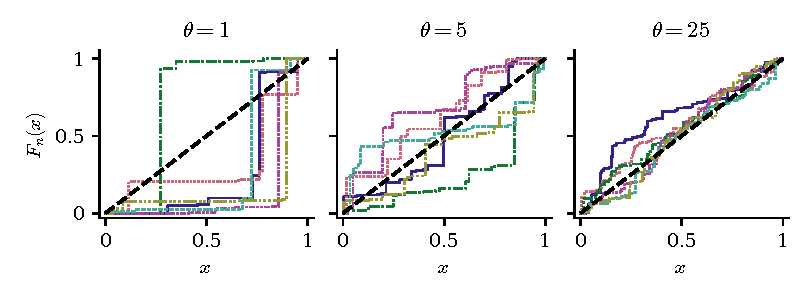
\includegraphics[width=\textwidth]{figures/esf_fig_cdfs.pdf}
\caption{Realisations of the empirical distribution function $F_{500}$ for $\theta \in \{1, 5, 25\}$ under the Ewens
predictive rule with $H$ uniform. The dashed line is $H$. The de Finetti measure $\mu$
is the law of the limit of these staircases.}
\label{esf:fig:cdfs}
\end{figure}

Figure \ref{esf:fig:var} plots the Monte Carlo variance of $F_{500}(x)$ against $x$
together with the exact curve $H(x)(1-H(x))(\theta+n)/\{n(1+\theta)\}$ of Proposition
\ref{esf:prop:exactvar}. The agreement is exact to simulation error at every $x$ and every
$\theta$, confirming the diagonal of the covariance kernel \eqref{esf:eq:kernel}.

\begin{figure}[htbp]
\centering
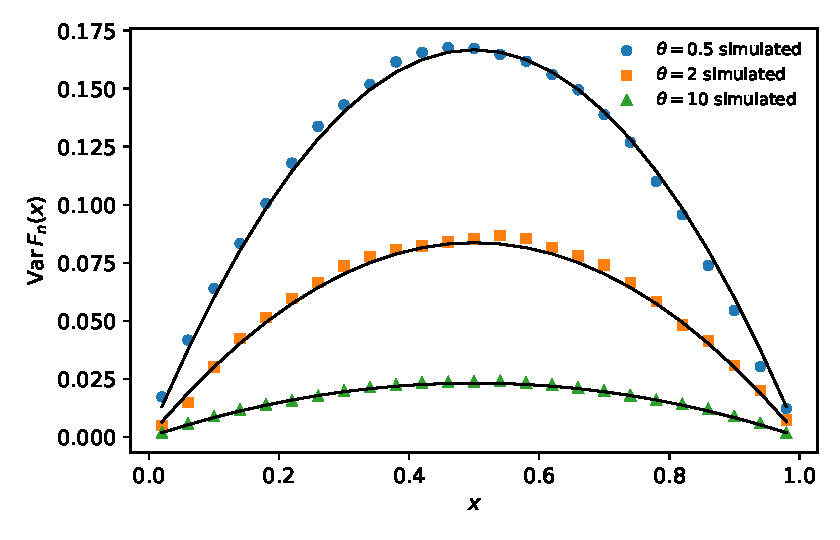
\includegraphics[width=0.75\textwidth]{figures/esf_fig_variance.pdf}
\caption{Variance of $F_n(x)$ at $n = 500$ from $1500$ replicates (markers) against
the exact formula \eqref{esf:eq:exactvar} (solid lines).}
\label{esf:fig:var}
\end{figure}

Table \ref{esf:tab:var} inverts the variance. The column headed $\hat\theta$ uses the
exact inversion \eqref{esf:eq:thetahat}; the column headed asymptotic uses the limiting
form \eqref{esf:eq:thetag}, which ignores the factor $(\theta+n)/n$. At $\theta = 10$ and
$n = 50$ the exact inversion returns $9.81$ while the asymptotic form returns $8.04$,
a twenty percent error that disappears only slowly.

\begin{table}[htbp]
\centering
\caption{Identifying $\theta$ from $\Var F_n(1/2)$, from $4000$ replicates with $H$
uniform. Exact variance from \eqref{esf:eq:exactvar}, exact inversion from
\eqref{esf:eq:thetahat}, asymptotic inversion from \eqref{esf:eq:thetag}.}
\label{esf:tab:var}
\begin{adjustbox}{max width=\textwidth}
\begin{tabular}{rrrrrr}
\toprule
$\theta$ & $n$ & $\Var F_n(1/2)$ & exact variance & $\hat\theta$ exact & $\hat\theta$ asymptotic \\
\midrule
0.5 &   50 & 0.16953 & 0.16833 & 0.489 & 0.475 \\
0.5 &  200 & 0.16878 & 0.16708 & 0.485 & 0.481 \\
0.5 & 5000 & 0.16564 & 0.16668 & 0.509 & 0.509 \\
2.0 &   50 & 0.08607 & 0.08667 & 2.022 & 1.905 \\
2.0 &  200 & 0.08257 & 0.08417 & 2.059 & 2.028 \\
2.0 & 5000 & 0.08248 & 0.08337 & 2.032 & 2.031 \\
10.0 &   50 & 0.02767 & 0.02727 & 9.809 & 8.036 \\
10.0 &  200 & 0.02418 & 0.02386 & 9.849 & 9.340 \\
10.0 & 5000 & 0.02268 & 0.02277 & 10.045 & 10.023 \\
\bottomrule
\end{tabular}
\end{adjustbox}
\end{table}

\subsection{The number of types}

Table \ref{esf:tab:kn} and Figure \ref{esf:fig:kn} illustrate Proposition \ref{esf:prop:kn}. The
predicted bias of $K_n/\log n$, namely $-\theta \psi(\theta)/\log n$, is confirmed to
within Monte Carlo error: at $n = 10^{4}$ the predicted values of $\E[K_n/\log n]$ are
$0.607$, $1.908$ and $7.556$ for $\theta = 0.5, 2, 10$, against simulated $0.607$,
$1.905$ and $7.572$. The maximum likelihood estimator is centred at the truth for $\theta \ge 2$ and for $n = 10^{4}$, but at $\theta = 0.5$ it is $15$ and $6$ percent too high at $n = 100$ and $n = 1000$, and its Monte Carlo standard deviation tracks $I_n(\theta)^{-1/2}$ closely. Note
how little the standard error improves between $n = 10^{3}$ and $n = 10^{4}$: this is
the $\log n$ information at work.

\begin{table}[htbp]
\centering
\caption{The number of types, $4000$ replicates, maximum likelihood over the first
$800$. The last column is the inverse root expected Fisher information.}
\label{esf:tab:kn}
\begin{adjustbox}{max width=\textwidth}
\begin{tabular}{rrrrrrrr}
\toprule
$\theta$ & $n$ & mean $K_n$ & $\E K_n$ & mean $K_n/\log n$ & mean $\hat\theta$ & sd $\hat\theta$ & $I_n^{-1/2}$ \\
\midrule
0.5 &   100 &  3.286 &  3.284 & 0.714 &  0.574 & 0.338 & 0.349 \\
0.5 &  1000 &  4.524 &  4.436 & 0.655 &  0.530 & 0.286 & 0.279 \\
0.5 & 10000 &  5.591 &  5.587 & 0.607 &  0.505 & 0.243 & 0.240 \\
2.0 &   100 &  8.393 &  8.395 & 1.822 &  2.037 & 0.870 & 0.827 \\
2.0 &  1000 & 12.987 & 12.973 & 1.880 &  2.035 & 0.642 & 0.620 \\
2.0 & 10000 & 17.550 & 17.575 & 1.905 &  2.012 & 0.511 & 0.516 \\
10.0 &   100 & 24.459 & 24.442 & 5.311 & 10.198 & 2.789 & 2.596 \\
10.0 &  1000 & 46.390 & 46.655 & 6.716 &  9.892 & 1.645 & 1.661 \\
10.0 & 10000 & 69.743 & 69.595 & 7.572 &  9.992 & 1.252 & 1.301 \\
\bottomrule
\end{tabular}
\end{adjustbox}
\end{table}

\begin{figure}[htbp]
\centering
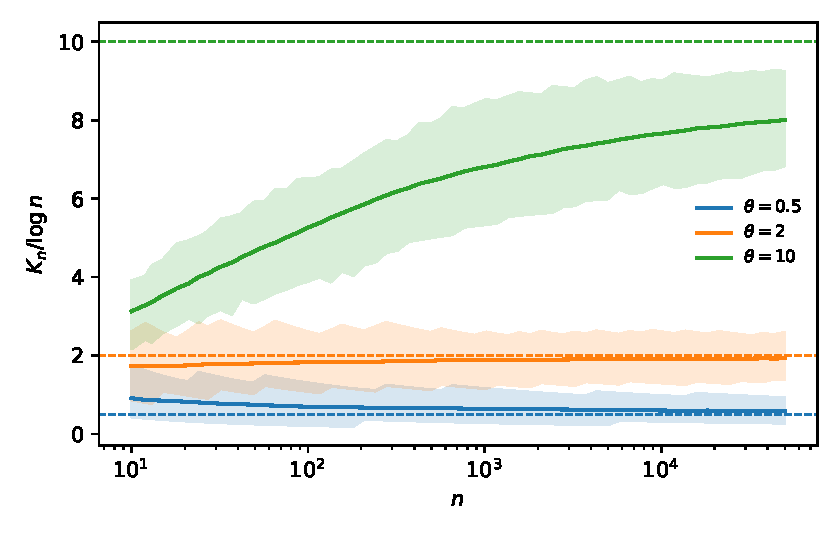
\includegraphics[width=0.75\textwidth]{figures/esf_fig_kn.pdf}
\caption{$K_n/\log n$ against $n$ on a logarithmic scale, mean and central ninety
percent band over $200$ paths. Dashed lines mark the true $\theta$. Convergence is at
rate $1/\log n$ and is slow for large $\theta$.}
\label{esf:fig:kn}
\end{figure}

\subsection{Corbet's Malayan butterflies}

We close with the data that prompted Fisher's logarithmic series, the abundances of
Malayan butterflies collected by Corbet and analysed in \citet{esf:fisher1943}. The collection held $620$ species, but the published table gives the abundance classes $j = 1, \dots, 24$ only, because Corbet took every individual seen of a species only until $24$ specimens had been taken \citep[p.~43]{esf:fisher1943}, so a count above $24$ is only a lower bound for the number seen and the classes above $24$ are censored by the collecting, not merely grouped. They comprise $501$ species and $3306$ individuals; the other $119$ species are known only to have more than $24$ individuals, and the total sample size $n$ is not reported. The data are therefore censored, and the likelihood is the probability under \eqref{esf:eq:esf} of the observed $a_1, \dots, a_{24}$ together with $119$ further blocks of size at least $25$ whose sizes sum to $n - 3306$. Summing \eqref{esf:eq:esf} over those blocks gives
\[
L(\theta, n) \;\propto\; \frac{\theta^{620}\, \Gamma(\theta)}{\Gamma(\theta+n)} \; n! \, \bigl[u^{\,n-3306}\bigr] \Bigl( \sum_{j \ge 25} \frac{u^{j}}{j} \Bigr)^{119} ,
\]
where $[u^m]$ extracts a coefficient. For fixed $n$ the likelihood depends on $\theta$ only through $K_n = 620$, so Proposition \ref{esf:prop:kn} still gives $\hat\theta$ given $n$, and $n$ is then profiled out, the coefficient being computed by exponential tilting and the fast Fourier transform. The result is
\[
\hat\theta = 141.75, \qquad \hat n = 11068, \qquad \text{standard error } 7.0,
\]
the standard error coming from the curvature of the profile likelihood of $\theta$. Fisher's own form of the model, in which the $A_j$ are independent Poisson variables with means $\theta x^{j}/j$ and $n$ is left random, gives $\hat\theta = 141.64$ on the same data. By Proposition \ref{esf:prop:moments} $\theta$ is also Fisher's $\alpha$, since the
logarithmic series approximation to $\E A_j$ agrees with the exact Ewens mean to within $0.013$
at every $j \le 24$ for these values of $n$ and $\theta$.

\begin{example}[Estimating $\theta$ for the butterflies]
\label{esf:ex:estimate}
The estimate $\hat\theta$ above is the estimator proposed by \citet{esf:ewens1972}:
solve $K_n = \E_\theta K_n$, which is at once the method of moments equation for the
sufficient statistic and, by Proposition \ref{esf:prop:kn}, the likelihood equation.
At the profiled sample size $n = 11068$, with $K_n = 620$, the score is
$s(\theta) = 620/\theta - \{\psi(\theta + 11068) - \psi(\theta)\}$ and the observed
information is $J(\theta) = 620/\theta^{2} - \{\psi'(\theta) - \psi'(\theta+11068)\}$.
Newton's method $\theta \leftarrow \theta + s(\theta)/J(\theta)$, started at the naive
value $K_n/\log n = 620/9.312 = 66.58$, gives
\[
66.58 \;\to\; 100.11 \;\to\; 128.50 \;\to\; 140.36 \;\to\; 141.73 \;\to\; 141.747
\;\to\; 141.747 ,
\]
converging in six steps. The starting value is off by a factor of more than two,
which is the bias $-\theta\psi(\theta)/\log n$ of Proposition \ref{esf:prop:kn} at work:
$\psi(142) \approx 4.95$, so $K_n/\log n$ estimates roughly
$\theta\{1 - 4.95/9.31\} \approx 0.47\,\theta$.

At $\hat\theta$ and $n = 11068$, $\Var K_n = 479.5$ and so, by \eqref{esf:eq:infovar},
$I_n(\hat\theta) = 479.5/141.7^{2} = 0.0239$ and the standard error given $n$ is
$0.0239^{-1/2} = 6.47$. Not knowing $n$ widens it to the $7.0$ of the profile likelihood. Two ninety five percent intervals agree closely: the Wald
interval $141.75 \pm 1.96 \times 7.0 = (128.0, 155.5)$, and the likelihood ratio interval, the set where
the profile log likelihood is within $1.92$ of its maximum, $(128.6, 156.0)$. The same profile puts $n$ between $9890$ and $12436$. The naive
asymptotic standard error $\sqrt{\theta/\log n} = 3.90$ is well below the correct value,
because $\log n$ is a poor proxy for $\sum_i i/(\theta+i)^{2}$ when $\theta$ is a
substantial fraction of $n$.

A different moment estimator uses the sample homozygosity, the proportion of pairs
of individuals of the same species,
\[
\hat F = \sum_{j} a_j \frac{j(j-1)}{n(n-1)}, \qquad \E \hat F = \frac{1}{1+\theta},
\qquad \hat\theta_F = \frac{1}{\hat F} - 1,
\]
the expectation following from $\PP(X_i = X_\ell) = 1/(1+\theta)$ for every pair. In
$2000$ simulated samples of $n = 11068$ from the urn at $\theta = 142$, with $n$ known, the maximum
likelihood estimator had mean $141.9$ and standard deviation $6.6$, matching
$I_n^{-1/2} = 6.47$, while $\hat\theta_F$ had mean $143.6$ and standard deviation
$16.4$. The homozygosity estimator, which ignores the sufficient statistic, has about
six times the variance of $\hat\theta$. Worse, as $n$ grows $\hat F$ converges not
to $1/(1+\theta)$ but to the random population homozygosity
$\sum_\ell p_\ell^{2} = \PP(X_1 = X_2 \mid \Ptil)$, so $\hat\theta_F$ is not even
consistent: no number of genes drawn from one population removes the variability of
that population's own frequencies. On
the butterfly table $\hat F$ cannot be computed at all: the homozygosity is dominated by the common
species, and the counts of the $119$ species with more than $24$ individuals were not recorded. The censoring removes $\hat F$ but leaves $K_n = 620$ intact, a further reason to
base inference on $K_n$.
\end{example}

Figure \ref{esf:fig:butterflies} and Table \ref{esf:tab:butterflies} show that the fit is fair but
misses in a specific direction. The model predicts $140.0$ singleton species and
$69.1$ doubletons; the data show $118$ and $74$. The rarest class is over predicted by
about a fifth, some two Poisson standard deviations, while the moderately abundant classes $j = 5, \dots, 12$ are under predicted, $151$ species against $131.0$ expected. The
expected counts over $j \le 24$ sum to $495.4$ against the observed $501$, leaving $124.6$ expected above $24$ against the observed $119$, and the Pearson discrepancy over the $24$ tabulated classes is $30.4$. The misfit is far milder than a fit that ignores the censoring suggests: treating the $24$ classes as the whole sample, with $n = 3306$ and $K_n = 501$, gives $\hat\theta = 163.99$, $156.3$ predicted singletons and a discrepancy of $100.5$. What remains is the pattern that ascertainment would produce. A model that fits the
tie structure of a simple random sample cannot simultaneously fit a collection in
which the rarest species are systematically less likely to be caught, and the observed sample may be a weighted, rather than a simple,
draw from the Kingman paintbox. Section \ref{esf:sec:weighted} formalises that idea, and
Section \ref{esf:sec:twoparam} enlarges the predictive rule; Section
\ref{esf:sec:butterflies2} returns to these data and reports which of the two mechanisms
the likelihood actually prefers.

\begin{table}[htbp]
\centering
\caption{Corbet's Malayan butterflies. Observed number of species with $j$
individuals, the exact Ewens mean \eqref{esf:eq:EAj} at $\hat\theta = 141.75$ and $\hat n = 11068$, and Fisher's
logarithmic series approximation. A further $119$ species have more than $24$ individuals.}
\label{esf:tab:butterflies}
\begin{adjustbox}{max width=\textwidth}
\begin{tabular}{rrrr rrrr}
\toprule
$j$ & observed & Ewens & log series & $j$ & observed & Ewens & log series \\
\midrule
 1 & 118 & 139.97 & 139.95 & 13 &  6 & 9.25 & 9.24 \\
 2 &  74 &  69.10 &  69.09 & 14 & 12 & 8.48 & 8.47 \\
 3 &  44 &  45.49 &  45.48 & 15 &  6 & 7.82 & 7.81 \\
 4 &  24 &  33.69 &  33.68 & 16 &  9 & 7.24 & 7.23 \\
 5 &  29 &  26.61 &  26.60 & 17 &  9 & 6.73 & 6.72 \\
 6 &  22 &  21.90 &  21.89 & 18 &  6 & 6.27 & 6.26 \\
 7 &  20 &  18.53 &  18.52 & 19 & 10 & 5.87 & 5.86 \\
 8 &  19 &  16.01 &  16.00 & 20 & 10 & 5.50 & 5.49 \\
 9 &  20 &  14.06 &  14.05 & 21 & 11 & 5.18 & 5.17 \\
10 &  15 &  12.49 &  12.48 & 22 &  5 & 4.88 & 4.87 \\
11 &  12 &  11.21 &  11.20 & 23 &  3 & 4.61 & 4.60 \\
12 &  14 &  10.15 &  10.14 & 24 &  3 & 4.36 & 4.35 \\
\bottomrule
\end{tabular}
\end{adjustbox}
\end{table}

\begin{figure}[htbp]
\centering
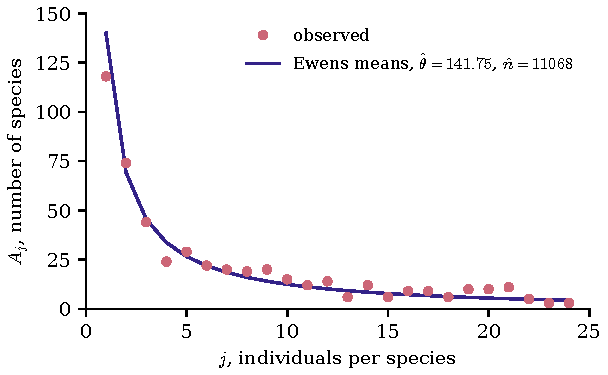
\includegraphics[width=0.75\textwidth]{figures/esf_fig_butterflies.pdf}
\caption{Corbet's Malayan butterflies: observed abundance counts against the fitted
Ewens means. The rarest class is over predicted and the moderately abundant classes
are under predicted, the pattern ascertainment would produce.}
\label{esf:fig:butterflies}
\end{figure}

\section{Ascertainment and the weighted paintbox}
\label{esf:sec:weighted}

\citet{esf:fisher1934} named the problem: a sample is rarely a simple random sample, because
the probability that an item enters the record may depend on the very quantity being
measured. \citet{esf:rao1965} gave the general device, the weighted distribution. We apply it
to Kingman's paintbox and ask what survives.

\subsection{The construction}

Let $P = (p_1 \ge p_2 \ge \cdots)$ be the ranked frequencies of the paintbox, so that
$\Ptil = \sum_{\ell \ge 1} p_\ell \delta_{\xi_\ell}$ with $\xi_\ell$ independent draws
from the diffuse $H$; under Proposition \ref{esf:prop:dp} the law of $P$ is Poisson
Dirichlet with parameter $\theta$. Let $w : (0,1] \to [0,\infty)$ be measurable with
$0 < \sum_\ell w(p_\ell) p_\ell < \infty$ almost surely.

\begin{definition}[Rao weighted paintbox]
The ascertained sample is a sequence $(X_i^w)_{i \ge 1}$ which, given $P$ and
$(\xi_\ell)$, is independent and identically distributed with common distribution
\begin{equation}
\Ptil^{\, w} \; = \; \frac{\sum_{\ell \ge 1} w(p_\ell) \, p_\ell \, \delta_{\xi_\ell}}
{\sum_{\ell \ge 1} w(p_\ell) \, p_\ell } .
\label{esf:eq:weighted}
\end{equation}
\end{definition}

The interpretation is that a species of relative abundance $p$ contributes to the
record in proportion to $w(p) p$ rather than to $p$: the collector's effort per
individual depends on how common that individual's species is. Taking $w$ increasing
represents a collector who overlooks rarities; $w$ decreasing represents a specialist
hunting them.

\begin{proposition}[The de Finetti architecture is invariant]
\label{esf:prop:invariant}
For every admissible $w$ the sequence $(X_i^w)$ is exchangeable, and Theorem
\ref{esf:thm:definetti} applies to it verbatim: the empirical distribution functions
$F_n^w$ converge almost surely and uniformly to a random distribution function, whose
law is the de Finetti measure, and that limit is the distribution function of
$\Ptil^{\, w}$. Only the mixing measure changes; Sections \ref{esf:sec:wor} and
\ref{esf:sec:helly} are untouched.
\end{proposition}

\begin{proof}
Conditionally on $(P, (\xi_\ell))$ the sequence is independent and identically
distributed, hence unconditionally exchangeable. Theorem \ref{esf:thm:definetti} was
proved for an arbitrary exchangeable sequence on $[0,1]$, so it applies, and the
uniqueness clause identifies the de Finetti measure with the law of the conditional
distribution, which is that of $\Ptil^{\, w}$.
\end{proof}

This is the point of interest for the present chapter. Helly selection and the Helly and
Bray lemma never used the Ewens hypothesis; they used only exchangeability. Weighting
can move the de Finetti measure off the Dirichlet process and so break the
sampling formula, but it does not touch the representation that produced the sampling
formula. What replaces \eqref{esf:eq:eppf} is the weighted paintbox partition function.

\begin{proposition}[Weighted exchangeable partition probability function]
\label{esf:prop:weppf}
The partition of $\{1,\dots,n\}$ induced by ties in $(X_i^w)$ is exchangeable with
\begin{equation}
p^{w}(n_1, \dots, n_k)
= \E \left[ \Bigl( \sum_{\ell} w(p_\ell) p_\ell \Bigr)^{-n}
\sum_{\ell_1, \dots, \ell_k \text{ distinct}}
\prod_{j=1}^{k} \bigl( w(p_{\ell_j}) p_{\ell_j} \bigr)^{n_j} \right],
\label{esf:eq:weppf}
\end{equation}
which reduces to \eqref{esf:eq:eppf} when $w$ is constant.
\end{proposition}

\begin{proof}
Condition on $P$ and $(\xi_\ell)$, use conditional independence and the fact that $H$
is diffuse, so that two observations are tied exactly when they land on the same
$\xi_\ell$, and sum over the assignment of blocks to distinct atoms. Constant $w$
cancels from numerator and denominator, leaving the Poisson Dirichlet paintbox, which
by Theorem \ref{esf:thm:esf} is the Ewens sampling formula.
\end{proof}

\subsection{Effort that ignores abundance is invisible}

Before fitting anything it is worth ruling out the simplest explanation of a misfit,
namely that the collector's effort varied over the collection period.

\begin{proposition}[Uniform thinning]
\label{esf:prop:thinning}
Let $\Pi_N$ follow the Ewens sampling formula with parameter $\theta$ and suppose each
of the $N$ indices is retained independently with probability $\pi \in (0,1]$, the
retention being independent of the types. Let $n$ be the number retained. Then,
conditionally on $n$, the partition of the retained indices follows the Ewens sampling
formula with the same $\theta$ and sample size $n$. The same holds if $\pi$ varies
across indices, provided it does not depend on the types.
\end{proposition}

\begin{proof}
The retained index set $R$ is independent of $(X_1,\dots,X_N)$, so conditionally on
$|R| = n$ the restricted sequence $(X_i)_{i \in R}$ is exchangeable with the same
finite dimensional laws as $(X_1,\dots,X_n)$. Its tie partition is therefore $\Pi_n$,
and Theorem \ref{esf:thm:esf} applies. This is Kingman's consistency, or deletion,
property: the Ewens family is a partition structure.
\end{proof}

Proposition \ref{esf:prop:thinning} says that a tired collector, one whose effort declines
over time but who is equally likely to miss a common and a rare specimen, produces
data indistinguishable from a smaller simple random sample. Any explanation of the
butterfly misfit must therefore involve dependence on abundance, which is exactly what
\eqref{esf:eq:weighted} supplies. A second negative result explains when the weighting must
break Assumption \ref{esf:as:pred}.

\begin{proposition}[Only a Dirichlet directing measure admits the affine predictive]
\label{esf:prop:zabell}
Among species sampling sequences, the affine predictive rule \eqref{esf:eq:pred} with
coefficients free of the data holds if and only if the directing measure is a
Dirichlet process. Consequently, if $w$ is not $P$ almost surely constant and $\Ptil^{\, w}$ is not a Dirichlet process, then
$(X_i^w)$ violates Assumption \ref{esf:as:pred}.
\end{proposition}

This is Johnson's sufficientness postulate in the form given by \citet{esf:zabell1982}, whose
argument requires the diffuse base measure assumed here; the forward direction is
Proposition \ref{esf:prop:weights} above. The stated consequence needs one further step,
that a nonconstant weighting actually moves $\Ptil^{\, w}$ off the Dirichlet process,
which we do not prove in general. For the power weights used below it is visible in
the simulations: at $\theta = 142$ and $\beta = 0.5$ the weighted paintbox produces
$308$ species with at most $24$ individuals at $n = 11068$, whereas the Ewens law with the same count ($\theta$ near $85.5$) gives about $85$ singletons and $42$ doubletons against the $89.5$ and $43.8$ of Table \ref{esf:tab:weighted}. It tells us where to look
for an enlargement: if we want tractability back, we must relax the predictive rule
itself rather than tinker with the weights, and Section \ref{esf:sec:twoparam} does so.

\subsection{What power weighting can and cannot do}

Take $w(p) = p^{\beta}$, so that the recorded frequencies are
$q_\ell \propto p_\ell^{1+\beta}$; $\beta = 0$ is simple random sampling and
$\beta > 0$ favours the abundant species. Table \ref{esf:tab:weighted} and Figure
\ref{esf:fig:weighted} report the abundance spectrum at $\theta = 142$ and $n = 11068$,
the values fitted to the butterflies, averaged over $60$ realisations of the
paintbox.

\begin{table}[htbp]
\centering
\caption{Power weighted paintbox, $\theta = 142$, $n = 11068$, $w(p) = p^{\beta}$,
$60$ replicates. Increasing $\beta$ suppresses the singletons and the richness in nearly the same proportion. The column $K_n$ counts the species represented by at most $24$ individuals, the quantity tabulated for the butterflies, so at $\beta = 0$ it is $497$ and not $\E K_n = 620$.}
\label{esf:tab:weighted}
\begin{adjustbox}{max width=\textwidth}
\begin{tabular}{rrrrrrr}
\toprule
$\beta$ & $A_1$ & $A_2$ & $A_5$ & $A_{10}$ & $A_{20}$ & $K_n$ \\
\midrule
0.00 & 139.3 & 70.9 & 26.2 & 12.9 & 5.8 & 496.9 \\
0.15 & 121.1 & 60.8 & 23.8 & 10.5 & 4.6 & 427.5 \\
0.30 & 108.1 & 52.6 & 20.1 &  9.1 & 4.0 & 368.7 \\
0.50 &  89.5 & 43.8 & 16.7 &  7.1 & 3.0 & 308.0 \\
\midrule
observed & 118 & 74 & 29 & 15 & 10 & 501 \\
\bottomrule
\end{tabular}
\end{adjustbox}
\end{table}

\begin{figure}[htbp]
\centering
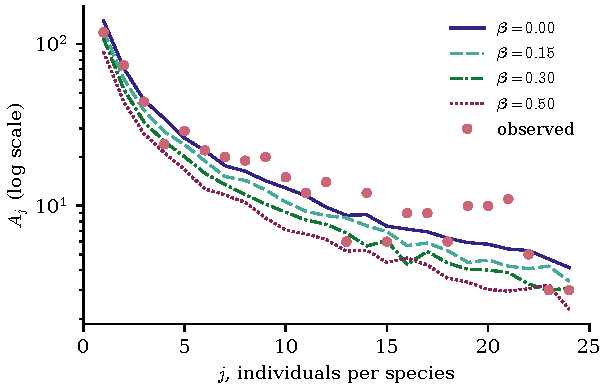
\includegraphics[width=0.75\textwidth]{figures/esf_fig_weighted.pdf}
\caption{Abundance spectra under the power weighted paintbox at $\theta = 142$ and $n = 11068$, on a logarithmic vertical
scale, against the observed butterfly counts.}
\label{esf:fig:weighted}
\end{figure}

The message is negative and useful. Raising $\beta$ does pull the singleton count down
from $139$ to the observed $118$ near $\beta = 0.2$, but it drags the number of species seen at most $24$ times down
with it, from $497$ to $308$ against an observed $501$, and it leaves the moderately
abundant classes too thin: $A_{20}$ falls from six to three where the data show
ten. A single tilt of the one parameter paintbox trades rare species against total
richness along a one dimensional curve, and the butterflies do not lie on it. The
data want more species and a flatter abundance profile at the same time, which is a
statement about the paintbox itself, not about how it is sampled.

\section{The two parameter family and a reanalysis}
\label{esf:sec:twoparam}

A weighted paintbox has no closed form partition function and, by Proposition
\ref{esf:prop:zabell}, no affine predictive rule. We take the other route: rather than
reweight a fixed paintbox, enlarge the predictive rule itself, in the smallest way
that keeps the empirical distribution function as the summary of the past. One extra
parameter buys back tractability.

\subsection{The predictive rule}

Assumption \ref{esf:as:pred} allowed the predictive law to load only two measures, the
base $H$ and the empirical distribution function $F_n$, with coefficients free of the
data. There is a third measure naturally available from $F_n$, namely the empirical
distribution function of its distinct jump locations,
\[
G_n(x) = \frac{1}{K_n} \sum_{\text{distinct values } v \le x} 1 ,
\]
which puts equal mass on each of the $K_n$ observed types regardless of how often each
was seen. Loading $G_n$ as well, and allowing the coefficients to depend on $K_n$,
gives the following relaxation.

\begin{assumption}[Two parameter predictive rule]
\label{esf:as:pred2}
With $H$ diffuse and $X_1 \sim H$, for every $n \ge 1$,
\begin{equation}
\PP\bigl(X_{n+1} \le x \mid X_1, \dots, X_n \bigr)
= \frac{\theta + \alpha K_n}{\theta + n} H(x)
\; + \; \frac{n}{\theta+n} F_n(x)
\; - \; \frac{\alpha K_n}{\theta+n} G_n(x),
\label{esf:eq:pypred}
\end{equation}
where either $0 \le \alpha < 1$ and $\theta > -\alpha$, or $\alpha < 0$ and
$\theta = m |\alpha|$ for an integer $m \ge 1$.
\end{assumption}

Equivalently, in urn form, index $n+1$ opens a new block with probability
$(\theta + \alpha K_n)/(\theta+n)$ and joins an existing block of current size $n_j$
with probability $(n_j - \alpha)/(\theta+n)$. Setting $\alpha = 0$ recovers
\eqref{esf:eq:bmq}. The coefficients still depend on the data only through the empirical
distribution function, now through its jump count as well as its heights, which is
precisely the relaxation of the sufficientness postulate studied by \citet{esf:zabell1997}. We
do not reprove the characterisation; we verify that \eqref{esf:eq:pypred} is exchangeable
by exhibiting its symmetric partition function.

\begin{theorem}[Pitman's sampling formula]
\label{esf:thm:py}
Under Assumption \ref{esf:as:pred2}, the tie partition of $\{1,\dots,n\}$
satisfies
\begin{equation}
\PP\bigl( \Pi_n = \{B_1,\dots,B_k\} \bigr)
= \frac{\prod_{i=1}^{k-1} (\theta + i \alpha)}{(\theta+1)_{n-1}}
\prod_{j=1}^{k} (1-\alpha)_{n_j - 1},
\label{esf:eq:pyeppf}
\end{equation}
where $(x)_m = x (x+1) \cdots (x+m-1)$ denotes the rising factorial,
and consequently
\begin{equation}
\PP(A_1 = a_1, \dots, A_n = a_n)
= n! \, \frac{\prod_{i=1}^{k-1}(\theta+i\alpha)}{(\theta+1)_{n-1}}
\prod_{j=1}^{n} \frac{1}{a_j!} \left( \frac{(1-\alpha)_{j-1}}{j!} \right)^{a_j},
\qquad k = \sum_j a_j .
\label{esf:eq:pysf}
\end{equation}
Both reduce to \eqref{esf:eq:eppf} and \eqref{esf:eq:esf2} at $\alpha = 0$.
\end{theorem}

\begin{proof}
Identical in structure to Proposition \ref{esf:prop:eppf} and Theorem \ref{esf:thm:esf}. Read
the indices in order. The denominator at step $i+1$ is $\theta+i$, giving
$\prod_{i=1}^{n-1}(\theta+i) = (\theta+1)_{n-1}$. The $i$th new block, for
$i = 1, \dots, k-1$, is opened when $i$ blocks are already present and contributes
$\theta + i \alpha$; the first block contributes nothing since index one opens it with
probability one. A block that ends with $n_j$ members contributes
$(1-\alpha)(2-\alpha)\cdots(n_j-1-\alpha) = (1-\alpha)_{n_j-1}$ as its second through
last members arrive. This gives \eqref{esf:eq:pyeppf}, which is symmetric in the block
sizes, so the partition is exchangeable. Multiplying by the number
$n!/\prod_j (j!)^{a_j} a_j!$ of set partitions with the given shape gives
\eqref{esf:eq:pysf}. At $\alpha = 0$, $\prod_{i=1}^{k-1}\theta = \theta^{k-1}$,
$(\theta+1)_{n-1} = \theta_{(n)}/\theta$ and $(1)_{n_j-1} = (n_j-1)!$.
\end{proof}

\begin{example}[Four genes under the two parameter rule]
\label{esf:ex:py4}
Take $n = 4$, so the denominator in \eqref{esf:eq:pyeppf} is
$(\theta+1)_3 = (\theta+1)(\theta+2)(\theta+3)$. Table \ref{esf:tab:py4} gives the five
shape probabilities for three parameter choices. For the single block at
$\alpha = 1/2$, $\theta = 1$, the product over new blocks is empty and the block
contributes $(1/2)_3 = \tfrac12 \cdot \tfrac32 \cdot \tfrac52 = 15/8$, so the
probability is $(15/8)/24 = 5/64$. Positive $\alpha$ moves mass towards many alleles:
$\E K_4 = 187/64 \approx 2.92$ against $25/12 \approx 2.08$ for the Ewens rule with the
same $\theta$. The choice $\alpha = -1$, $\theta = 2$ is the finite pool of Remark
\ref{esf:rem:finite} with $m = 2$ types, the frequency of the first type being uniform
on $[0,1]$: the factor
$\theta + 2\alpha = 0$ kills every partition with three or more blocks, and the
remaining three probabilities $2/5, 2/5, 1/5$ can be checked directly, since with
$P \sim \mathrm{Beta}(1,1)$ a given sequence with $c$ genes of the first type has
probability $\int_0^1 p^{c}(1-p)^{4-c}\,dp = c!\,(4-c)!/5!$; for instance the shape $4$
has probability $2 \cdot 4!/5! = 2/5$.
\end{example}

\begin{table}[htbp]
\centering
\caption{The two parameter partition law at $n = 4$. The column $N$ is the number of
set partitions with the given shape.}
\label{esf:tab:py4}
\begin{adjustbox}{max width=\textwidth}
\begin{tabular}{lrrrr}
\toprule
Shape & $N$ & $\alpha = 1/2,\ \theta = 1$ & $\alpha = 0,\ \theta = 1$ & $\alpha = -1,\ \theta = 2$ \\
\midrule
$4$       & 1 & $5/64$  & $1/4$  & $2/5$ \\
$3+1$     & 4 & $3/16$  & $1/3$  & $2/5$ \\
$2+2$     & 3 & $3/64$  & $1/8$  & $1/5$ \\
$2+1+1$   & 6 & $3/8$   & $1/4$  & $0$ \\
$1+1+1+1$ & 1 & $5/16$  & $1/24$ & $0$ \\
\midrule
$\E K_4$  &   & $187/64$ & $25/12$ & $8/5$ \\
\bottomrule
\end{tabular}
\end{adjustbox}
\end{table}

\begin{proposition}[Exact abundance means]
\label{esf:prop:pyEA}
Under \eqref{esf:eq:pysf}, for $1 \le j \le n$,
\begin{equation}
\E A_j = \binom{n}{j} \,
\frac{(1-\alpha)_{j-1} \, (\theta + \alpha)_{n-j}}
{(\theta+1)_{n-1}} ,
\label{esf:eq:pyEA}
\end{equation}
which reduces to \eqref{esf:eq:EAj} at $\alpha = 0$.
\end{proposition}

\begin{proof}
By exchangeability $\E A_j = \binom{n}{j} \PP(B)$ where $B$ is the event that
$\{1,\dots,j\}$ is a block of $\Pi_n$. Summing \eqref{esf:eq:pyeppf} over all partitions
of the remaining $n-j$ indices into blocks of sizes $m_1,\dots,m_r$, the summand is
\[
\frac{\prod_{i=1}^{r}(\theta+i\alpha)}{(\theta+1)_{n-1}} (1-\alpha)_{j-1}
\prod_{i=1}^{r} (1-\alpha)_{m_i - 1}
\]
\[
\qquad = \; \frac{(\theta+\alpha) (1-\alpha)_{j-1} (\theta+\alpha+1)_{n-j-1}}
{(\theta+1)_{n-1}} \times p_{\alpha, \theta+\alpha}(m_1,\dots,m_r),
\]
because $\prod_{i=1}^{r}(\theta+i\alpha) = (\theta+\alpha)
\prod_{i=1}^{r-1}(\theta+\alpha+i\alpha)$. The second factor is the partition function
\eqref{esf:eq:pyeppf} for the two parameter family with parameters $(\alpha, \theta+\alpha)$
on $n-j$ indices, and it sums to one over all such partitions. Since $(\theta+\alpha)(\theta+\alpha+1)_{n-j-1} = (\theta+\alpha)_{n-j}$, this gives \eqref{esf:eq:pyEA} for $j < n$; for $j = n$ the event $B$ is the single block partition, whose probability $(1-\alpha)_{n-1}/(\theta+1)_{n-1}$ gives \eqref{esf:eq:pyEA} with $(\theta+\alpha)_0 = 1$. At $\alpha = 0$ the
constant becomes $\theta (j-1)! \, \Gamma(\theta+n-j)/\Gamma(\theta+n)$, which is
\eqref{esf:eq:EAj}.
\end{proof}

\subsection{What the empirical distribution function identifies}

\begin{proposition}[Second order structure and what it identifies]
\label{esf:prop:pyident}
Under Assumption \ref{esf:as:pred2}, write $\rho = (1-\alpha)/(1+\theta)$. Then
$\PP(X_1 = X_2) = \rho$ and, for every $g \in L^2(H)$ and every $n$,
\begin{equation}
\Var \left( \int g \, d\Ptil \right) = \rho \, \Var_H(g),
\qquad
\Var \left( \int g \, dP_n \right)
= \Var_H(g) \left\{ \frac{1}{n} + \frac{n-1}{n} \rho \right\},
\label{esf:eq:pyvar}
\end{equation}
and $\Cov(\Ftil(x), \Ftil(y)) = \rho \{ H(x \wedge y) - H(x) H(y) \}$. Hence the
covariance kernel of the Helly and Bray limit identifies only the single number
$\rho$, and not the pair $(\alpha, \theta)$. The two are separated by the growth of
the number of jumps of $F_n$:
\[
\frac{K_n}{\log n} \to \theta \ \ (\alpha = 0), \qquad
\frac{K_n}{n^{\alpha}} \to S_\alpha \ \ (0 < \alpha < 1), \qquad
K_n \uparrow m \ \ (\alpha < 0),
\]
almost surely, where $S_\alpha$ is a strictly positive random variable.
\end{proposition}

\begin{proof}
The predictive rule at $n=1$ gives $\PP(X_2 = X_1) = (1-\alpha)/(\theta+1) = \rho$,
since the single existing block has size one. The proofs of Propositions
\ref{esf:prop:cov} and \ref{esf:prop:exactvar} used only the value of this tie probability,
through $\Cov(g(X_1),g(X_2)) = \rho \Var_H(g)$, so they carry over with
$1/(1+\theta)$ replaced by $\rho$. Any $(\alpha,\theta)$ on the line $1 - \alpha =
\rho(1+\theta)$ therefore gives the same de Finetti covariance kernel. The three limit
laws for $K_n$ are classical: for $\alpha = 0$ it follows from the independent indicators in the proof of Proposition \ref{esf:prop:kn} and the strong law for independent summands, for
$\alpha>0$ it is the law of large numbers of \citet{esf:pitmanyor1997}, and for $\alpha<0$ the number of
types is bounded above by $m$ and reaches it almost surely.
\end{proof}

Proposition \ref{esf:prop:pyident} sharpens the theme of the chapter. The limiting empirical
distribution function identifies the model through exactly two functionals of a
different character: the variance of its heights, which gives $\rho$, and the growth
rate of the number of its jumps, which gives $\alpha$. In the Ewens case the second
functional is degenerate, $\alpha = 0$ is known, and the first suffices; that is why
Section \ref{esf:sec:ident} could identify $\theta$ from a single moment.

\begin{remark}[The negative branch is a finite species pool]
\label{esf:rem:finite}
When $\alpha < 0$ and $\theta = m|\alpha|$, the directing random measure is
$\Ptil = \sum_{i=1}^{m} P_i \delta_{\xi_i}$ with
$(P_1,\dots,P_m) \sim \Dir(|\alpha|,\dots,|\alpha|)$ symmetric on $m$ types, and
\eqref{esf:eq:pysf} is the Dirichlet multinomial partition law. The urn of Assumption
\ref{esf:as:pred2} then closes: once $K_n = m$ the probability of a new type is
$(\theta+m\alpha)/(\theta+n) = 0$. This branch is not an ascertainment model at all;
it is a statement that the pool of species is finite, of size $m$, with a symmetric
Dirichlet abundance profile of concentration $|\alpha|$.
\end{remark}

\begin{remark}[Weighting and tilting are different operations]
On the negative branch the two parameter family is not the weighted paintbox \eqref{esf:eq:weighted} of the one
parameter family for any choice of $\theta$ and $w$; Proposition \ref{esf:prop:notweighted} below proves it. For $0 < \alpha < 1$ we do not know whether some weight reproduces the two parameter law exactly: a growth rate argument does not exclude it, since a weight with $w(p)\,p$ of order $(\log 1/p)^{-1/\alpha}$ turns the geometric decay of the ranked Poisson Dirichlet frequencies into the power decay of the two parameter family, and we record the question in Section \ref{esf:sec:discussion}. For $0 < \alpha < 1$ the two parameter family arises instead from a tilt of the stable
subordinator that generates the frequencies \citep{esf:perman1992,esf:pitmanyor1997}, which changes the law of $P$ itself
rather than reweighting a fixed $P$. The two mechanisms are genuinely distinct
hypotheses about the same data, and Sections \ref{esf:sec:weighted} and \ref{esf:sec:butterflies2} compare them
informally on the butterflies.
\end{remark}

\begin{proposition}[The negative branch is not a weighted paintbox]
\label{esf:prop:notweighted}
Let $\alpha < 0$ and $\theta = m|\alpha|$ with $m$ a positive integer. For no $\theta' > 0$ and no admissible weight $w$ is the weighted paintbox \eqref{esf:eq:weighted} built on Poisson Dirichlet frequencies with parameter $\theta'$ equal in law to the two parameter paintbox with parameters $(\alpha, \theta)$.
\end{proposition}

\begin{proof}
Let $S = \{p \in (0,1] : w(p) > 0\}$ and, for $0 < r \le 1$, let $N_r = \#\{\ell : r p_\ell \in S\}$. Since the $\xi_\ell$ are distinct, $\Ptil^{\, w}$ has exactly $N_1$ atoms, while by Remark \ref{esf:rem:finite} the two parameter paintbox has exactly $m$; so it suffices to show that $N_1 = m$ almost surely is impossible. By the stick breaking construction \citep{esf:pitmanyor1997}, the frequencies are $V$ together with $(1-V)$ times the frequencies $P'$ of an independent Poisson Dirichlet paintbox with parameter $\theta'$, where $V \sim \mathrm{Beta}(1,\theta')$ has a positive density on $(0,1)$. Hence $N_r = \mathbf{1}_S(rV) + N'_{r(1-V)}$, with $N'$ computed from $P'$. If $N_1 = m$ almost surely then, by Fubini's theorem, $N'_{1-v}$ is almost surely constant for almost every $v$, so there is a function $g$ with $N_r = g(r)$ almost surely for almost every $r \in (0,1)$; applying the same decomposition to such an $N_r$ gives $g(r) = \mathbf{1}_S(rv) + g(r(1-v))$ for almost every $(r, v) \in (0,1)^2$. In the variables $u = rv$ and $s = r(1-v)$ this reads $g(u+s) = \mathbf{1}_S(u) + g(s)$ for almost every $(u,s)$ with $u + s < 1$. Expanding $g(u+s+t)$ once as $\mathbf{1}_S(u+s) + g(t)$ and once as $\mathbf{1}_S(u) + \mathbf{1}_S(s) + g(t)$ yields
\[
\mathbf{1}_S(u+s) = \mathbf{1}_S(u) + \mathbf{1}_S(s) \quad \text{for almost every } (u,s) \text{ with } u + s < 1 .
\]
The left side is at most one, so $S \cap (0,\tfrac12)$ is a null set; then the right side vanishes for almost every $u, s \in (0, \tfrac12)$, and since $u + s$ has a positive density on $(0,1)$ when $u$ and $s$ are independent and uniform on $(0,\tfrac12)$, $S \cap (0,1)$ is a null set. The atom sizes are almost surely smaller than one and their intensity $\theta' x^{-1}(1-x)^{\theta'-1}\,dx$ is absolutely continuous, so $N_1 = 0$ almost surely, which contradicts $m \ge 1$ (and the admissibility condition $\sum_\ell w(p_\ell)p_\ell > 0$).
\end{proof}

\subsection{The butterflies revisited}
\label{esf:sec:butterflies2}

We now refit Corbet's data, $620$ species of which $119$ are censored above $24$ individuals, under
\eqref{esf:eq:pysf}. The censored likelihood is built as in Section \ref{esf:sec:empirical}, with the weight $1/j$ of a block of size $j$ replaced by $(1-\alpha)_{j-1}/j!$ and $\theta^{620}\Gamma(\theta)/\Gamma(\theta+n)$ by $\prod_{i=1}^{619}(\theta+i\alpha)/(\theta+1)_{n-1}$, and $n$ is again profiled out. Unlike the Ewens case, the two parameter likelihood depends on the
whole vector $(a_1, \dots, a_{24})$ and not only on $K_n$, since the sufficiency of
Corollary \ref{esf:cor:suff} is a property of the one parameter family alone. Maximising it numerically gives the results in Table \ref{esf:tab:fits}; the log likelihoods are those of the censored data, constants included.

\begin{table}[htbp]
\centering
\caption{Fits to Corbet's Malayan butterflies. The two parameter maximum lies on the
negative $\alpha$ branch; restricted to $\alpha \ge 0$ the maximum is attained at the
Ewens boundary $\alpha = 0$.}
\label{esf:tab:fits}
\begin{adjustbox}{max width=\textwidth}
\begin{tabular}{lrrrrr}
\toprule
Model & $\hat\alpha$ & $\hat\theta$ & $\hat n$ & log likelihood & Pearson discrepancy \\
\midrule
Ewens, $\alpha = 0$        & 0      & 141.75 & 11068 & $-70.13$ & 30.4 \\
Two parameter, $\alpha \ge 0$ & 0.000  & 141.75 & 11068 & $-70.13$ & 30.4 \\
Two parameter, unrestricted  & $-0.1454$ & 209.70 & 9747 & $-65.85$  & 20.0 \\
\bottomrule
\end{tabular}
\end{adjustbox}
\end{table}

Three things are worth drawing out.

First, the likelihood moves to the negative branch. The improvement in log
likelihood is $4.3$, a likelihood ratio statistic of $8.57$; since $\alpha = 0$ is an interior point of the range searched, the reference distribution is chi squared on one degree of freedom, whose ninety nine percent point is $6.63$, so the evidence is clear though far from overwhelming. Ignoring the censoring, with $n = 3306$ and $K_n = 501$, exaggerates it: that fit gives $\hat\alpha = -0.49$ and a statistic of $44.3$. By
Remark \ref{esf:rem:finite} the fitted model is a finite pool of
$\hat m = \hat\theta / |\hat\alpha| = 1443$ species with a symmetric Dirichlet
abundance profile of concentration $0.15$. The optimisation treated $m$ as continuous; the model is proper only at integer $m$, and the likelihood is flat
enough at this scale that the rounding is immaterial. The data are not saying that rare
butterflies were overlooked; they are saying that the pool of species is finite, of the order of twice the $620$ already seen.

Second, the fit to the rare classes improves in exactly the place the diagnostics
pointed. The predicted singleton count falls from $140.0$ to $117.1$ against an
observed $118$, the doubletons move from $69.1$ to $65.7$ against $74$, and the
Pearson discrepancy $\sum_j (A_j - \E A_j)^2 / \E A_j$ over the tabulated classes
falls from $30.4$ to $20.0$. That quantity is descriptive only: the cells are
dependent, being counts of a single partition, and the expected values do not sum to
the observed total, so it should not be referred to a chi squared distribution. Table
\ref{esf:tab:butterflies2} and Figure \ref{esf:fig:butterflies2} give the detail. The
remaining misfit lies largely in the classes $j = 19$ to $24$: the data show $31$ species in classes $19$ to $21$ against $19.4$ expected under the two parameter fit, and $11$ in classes $22$ to $24$ against $16.2$, an irregularity that neither model reproduces.

\begin{table}[htbp]
\centering
\caption{Corbet's butterflies: observed counts against the exact means \eqref{esf:eq:EAj}
and \eqref{esf:eq:pyEA} at the fitted parameters, each at its own $\hat n$.}
\label{esf:tab:butterflies2}
\begin{adjustbox}{max width=\textwidth}
\begin{tabular}{rrrr rrrr}
\toprule
$j$ & observed & Ewens & two parameter & $j$ & observed & Ewens & two parameter \\
\midrule
 1 & 118 & 139.97 & 117.09 & 13 &  6 & 9.25 & 10.80 \\
 2 &  74 &  69.10 &  65.65 & 14 & 12 & 8.48 &  9.93 \\
 3 &  44 &  45.49 &  45.96 & 15 &  6 & 7.82 &  9.17 \\
 4 &  24 &  33.69 &  35.39 & 16 &  9 & 7.24 &  8.49 \\
 5 &  29 &  26.61 &  28.72 & 17 &  9 & 6.73 &  7.90 \\
 6 &  22 &  21.90 &  24.12 & 18 &  6 & 6.27 &  7.36 \\
 7 &  20 &  18.53 &  20.73 & 19 & 10 & 5.87 &  6.89 \\
 8 &  19 &  16.01 &  18.13 & 20 & 10 & 5.50 &  6.45 \\
 9 &  20 &  14.06 &  16.06 & 21 & 11 & 5.18 &  6.06 \\
10 &  15 &  12.49 &  14.38 & 22 &  5 & 4.88 &  5.70 \\
11 &  12 &  11.21 &  12.98 & 23 &  3 & 4.61 &  5.38 \\
12 &  14 &  10.15 &  11.81 & 24 &  3 & 4.36 &  5.08 \\
\bottomrule
\end{tabular}
\end{adjustbox}
\end{table}

\begin{figure}[htbp]
\centering
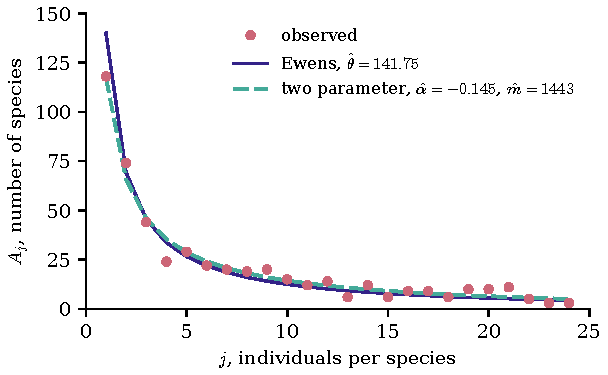
\includegraphics[width=0.75\textwidth]{figures/esf_fig_butterflies2.pdf}
\caption{Corbet's Malayan butterflies with the one and two parameter fits. The
negative $\alpha$ fit corrects the over prediction of singletons and lifts the middle
of the spectrum.}
\label{esf:fig:butterflies2}
\end{figure}

Third, the choice of branch matters for the question Corbet actually asked Fisher, how
many new species a second two year expedition would yield. Taking a second sample of the same size $\hat n$ as each fit, and computing the expected number of species in the combined sample of $2\hat n$ given the $620$ already seen, gives
\[
\text{Ewens: } 97.4 \ \text{new species}, \qquad
\text{two parameter: } 77.7 ,
\]
against the model free alternating sum of \citet{esf:good1956} evaluated on the
tabulated classes, $\sum_{j=1}^{24} (-1)^{j+1} A_j = 75$, which is the figure Fisher reported (the terms with $j > 24$ are unknown, and under either fit their expected contribution is small, about two species under the Ewens fit).
The one parameter model is the optimistic one, as it must be: with $\alpha = 0$ the
species pool is inexhaustible and $K_n$ grows without bound like $\theta \log n$,
whereas the fitted negative branch has seen $620$ of a ceiling of about
$1443$ and grows more slowly. The nonparametric answer lies close to the two parameter one and well below the Ewens one.

\begin{remark}[Caveats]
Two should be recorded. First, the tabulation used here is the published one, censored at
$j = 24$, and the fits use only the fact, reported by \citet{esf:fisher1943}, that $119$ further species had more than $24$ individuals; the total $n$ is estimated, not observed, and an analysis that treats the $24$ classes as the whole sample overstates both the misfit of the Ewens model and the evidence for the negative branch. The fitted $\theta$
of $142$ should not be compared with the value near $40$ that is often quoted for
Fisher's $\alpha$, since the latter belongs to the Rothamsted light trap moths, a
different data set with $240$ species and about $15{,}600$ individuals. Second,
Proposition \ref{esf:prop:weppf} and Theorem \ref{esf:thm:py} are not nested, so the
comparison in Table \ref{esf:tab:fits} is between the two parameter family and the Ewens
submodel, not between weighting and tilting; the weighted paintbox is ruled out here
informally, by Table \ref{esf:tab:weighted}, rather than by a likelihood ratio.
\end{remark}

\section{The Kingman coalescent}
\label{esf:sec:coalescent}

The derivation above makes no reference to genealogy, which invites an obvious
objection: the Ewens sampling formula is usually, and most naturally, obtained from
Kingman's coalescent \citep{esf:kingman1982a,esf:kingman1982b}, where it falls out of the
genealogical process directly \citep{esf:griffiths1979,esf:ewens2004}. This section sets the
two derivations side by side. The relationship is closer than it first appears, and
looking at it settles which of the two arguments assumes what.

\subsection{The coalescent with killing is the predictive rule}

Consider the standard construction. Trace the ancestry of a sample of $n$ genes
backwards in time under the infinitely many alleles model: each pair of ancestral
lineages coalesces at rate one, and each lineage mutates at rate $\theta/2$, a
mutation conferring an allele never seen before and resolving the type of every sample
member below it. Every event, coalescence or mutation, reduces the number of active
lineages by one, so the construction terminates after exactly $n$ events.

\begin{proposition}[The competing exponentials give the predictive weights]
\label{esf:prop:coal}
With $m$ active lineages, the probability that the next event backwards in time is a
mutation rather than a coalescence is
\begin{equation}
\frac{m \theta / 2}{\binom{m}{2} + m \theta / 2}
= \frac{\theta}{\theta + m - 1},
\label{esf:eq:coalrates}
\end{equation}
and the complementary probability of a coalescence is $(m-1)/(\theta+m-1)$. Setting
$m = n+1$, these are exactly the weights $c_n = \theta/(\theta+n)$ and $1 - c_n$ of
Proposition \ref{esf:prop:weights}.
\end{proposition}

\begin{proof}
The total coalescence rate among $m$ lineages is $\binom{m}{2} = m(m-1)/2$ and the
total mutation rate is $m\theta/2$; the ratio of competing exponential rates gives
\eqref{esf:eq:coalrates} after cancelling $m/2$.
\end{proof}

\begin{example}[Three genes traced back by hand]
\label{esf:ex:coal3}
Start with three lineages. The first event is a mutation with probability
$\theta/(\theta+2)$ and a coalescence with probability $2/(\theta+2)$.

If it is a coalescence, two of the genes now share one ancestral lineage, and two
lineages remain. The next event is a coalescence with probability $1/(\theta+1)$, in
which case all three genes descend from one lineage and carry one allele whatever
happens later; or a mutation with probability $\theta/(\theta+1)$, which separates the
two lineages for good and produces the shape $2+1$.

If the first event is a mutation, the gene on that lineage carries an allele no other
sample member shares, and two lineages remain; they coalesce next with probability
$1/(\theta+1)$, giving shape $2+1$, or mutate with probability $\theta/(\theta+1)$,
giving three distinct alleles. Collecting the paths,
\[
\begin{aligned}
\PP(\text{shape } 3) &= \frac{2}{\theta+2}\cdot\frac{1}{\theta+1}
= \frac{2}{(\theta+1)(\theta+2)}, \\
\PP(\text{shape } 2+1) &= \frac{2}{\theta+2}\cdot\frac{\theta}{\theta+1}
+ \frac{\theta}{\theta+2}\cdot\frac{1}{\theta+1}
= \frac{3\theta}{(\theta+1)(\theta+2)}, \\
\PP(\text{shape } 1+1+1) &= \frac{\theta}{\theta+2}\cdot\frac{\theta}{\theta+1}
= \frac{\theta^{2}}{(\theta+1)(\theta+2)} .
\end{aligned}
\]
These are exactly \eqref{esf:eq:esfcycle} at $n = 3$, with $c(a) = 2, 3, 1$ and
$\theta_{(3)} = \theta(\theta+1)(\theta+2)$; they sum to
$(\theta^2 + 3\theta + 2)/\{(\theta+1)(\theta+2)\} = 1$. At $\theta = 1$ they are
$1/3, 1/2, 1/6$, the cycle type probabilities of a random permutation of three
objects. The urn produces the same numbers forwards in time: the factors
$1/(\theta+1)$ and $2/(\theta+2)$ are the joining probabilities for the second and
third genes.
\end{example}

So Hoppe's urn is the killed coalescent read backwards, one event at a time: adding
the $(n+1)$st observation to the urn corresponds to removing one of $n+1$ lineages
from the genealogy, a new colour corresponding to a mutation and a repeated colour to
a coalescence. That the allelic partition of the killed coalescent is the Ewens
sampling formula is classical \citep{esf:kingman1982b,esf:griffiths1979}, and we do not
reprove it; Table \ref{esf:tab:coal} instead reports a direct simulation of the genealogy,
with the pair chosen uniformly at each coalescence, checked against \eqref{esf:eq:esf2}.

\begin{table}[htbp]
\centering
\caption{Allelic partitions from simulating the coalescent with killing, against the
Ewens sampling formula \eqref{esf:eq:esf2}. Each row is $200{,}000$ independent
genealogies; the statistic is the chi squared goodness of fit over all observed
partition shapes.}
\label{esf:tab:coal}
\begin{adjustbox}{max width=\textwidth}
\begin{tabular}{rrrrr}
\toprule
$n$ & $\theta$ & shapes observed & chi squared & degrees of freedom \\
\midrule
 6 & 0.5 & 11 &  8.5 & 10 \\
 8 & 2.0 & 22 & 24.7 & 21 \\
10 & 5.0 & 42 & 57.0 & 41 \\
\bottomrule
\end{tabular}
\end{adjustbox}
\end{table}

\subsection{Which way the implication runs}

The genealogical argument and the present one use the same arithmetic in opposite
directions, and that is the substantive point. The coalescent derivation posits a
population model, extracts the rates, and deduces the predictive weights; $\theta$
enters as a ratio of rates, $\theta = 4N\mu$, four times the product of the diploid
population size $N$ and the mutation rate $\mu$ per gene per generation, and is a
modelling input. Proposition \ref{esf:prop:weights} runs the other way. It
assumes nothing about time, population size, reproduction or mutation. It assumes only
that the sample is exchangeable and that the one step forecast is affine in the
empirical distribution function, and it then forces $c_n = \theta/(\theta+n)$ using
nothing beyond the equality of pairwise tie probabilities. The competing exponential
structure of the coalescent is therefore not needed to obtain the Ewens formula: it is
implied by exchangeability together with predictive sufficiency of $F_n$.

The parameter changes character in the same way. Genealogically $\theta$ is a rate
ratio; here, by Propositions \ref{esf:prop:cov} and \ref{esf:prop:exactvar}, it is
\[
\theta = \frac{1-q}{q} = \frac{\Var_H(g)}{\Var \bigl( \int g \, d\Ptil \bigr)} - 1 ,
\]
where $q = \PP(X_1 = X_2)$ is the homozygosity, so that a ratio of rates in the
genealogy is a ratio of variances of the limiting empirical distribution function.

This cuts both ways, and the negative half is worth stating plainly. Any mechanism
whatever that delivers the predictive rule \eqref{esf:eq:bmq} delivers the Ewens sampling
formula, so the allelic partition of a sample carries no information about the
genealogy beyond that rule. The sampling formula cannot be used to confirm the
coalescent; it can only fail to contradict it.

\subsection{Why the information grows like a logarithm}

The genealogy does explain something the urn leaves mysterious, namely the very slow
information growth of Proposition \ref{esf:prop:kn}. Mutations fall on the coalescent tree
as a Poisson process of rate $\theta/2$ per unit length, so the information about
$\theta$ should be proportional to the expected total branch length
\[
\E L_n = 2 \sum_{k=1}^{n-1} \frac{1}{k} ,
\]
and indeed
\begin{equation}
I_n(\theta) = \frac{\E L_n}{2 \theta} + O(1) ,
\label{esf:eq:infolength}
\end{equation}
the two sides differing by a constant that depends on $\theta$ alone: numerically the
difference settles at $2.162$, $1.145$ and $0.388$ for $\theta = 0.5, 2, 10$, stable
to three decimal places between $n = 10^{4}$ and $n = 10^{6}$.

Both halves of this statement can be checked directly. While $k$ lineages remain in
the coalescent without mutation, the waiting time $T_k$ to the next coalescence is
exponential with rate $\binom{k}{2}$, and those $k$ lineages contribute $k T_k$ to the
total length, so
\[
\E L_n = \sum_{k=2}^{n} k \, \E T_k = \sum_{k=2}^{n} \frac{2}{k-1}
= 2 \sum_{k=1}^{n-1} \frac{1}{k} .
\]
For the difference, $\E L_n/(2\theta) = \theta^{-1}\sum_{i=1}^{n-1} i^{-1}$ and
$I_n(\theta) = \sum_{i=1}^{n-1} i/\{\theta(\theta+i)^{2}\}$, so
\begin{equation}
\frac{\E L_n}{2\theta} - I_n(\theta)
= \frac{1}{\theta}\sum_{i=1}^{n-1} \left\{ \frac{1}{i} - \frac{i}{(\theta+i)^{2}} \right\}
= \sum_{i=1}^{n-1} \frac{2i + \theta}{i\,(\theta+i)^{2}} ,
\label{esf:eq:infogap}
\end{equation}
a series of positive terms of order $2/i^{2}$. It increases to a finite limit
$c(\theta)$, which is $2.162$, $1.145$ and $0.388$ at $\theta = 0.5, 2, 10$, and this
proves \eqref{esf:eq:infolength}.

Why compare with $\E L_n / (2\theta)$ at all? Suppose an oracle revealed the tree and
the number $S_n$ of mutations on it, as the infinitely many sites model would. Given
the tree, $S_n$ is Poisson with mean $\theta L_n/2$, whose Fisher information about
$\theta$ is $(L_n/2)/\theta$, with expectation $\E L_n/(2\theta)$. So
\eqref{esf:eq:infolength} says that the allelic partition carries all but a bounded
amount of the information that the full tree and its mutations would carry, and
\eqref{esf:eq:infogap} measures exactly what is lost by seeing only which genes share
an allele.

\begin{example}[Four genes]
\label{esf:ex:tree4}
For $n = 4$, $\E T_4 = 1/6$, $\E T_3 = 1/3$ and $\E T_2 = 1$, so
$\E L_4 = 4/6 + 3/3 + 2 = 11/3$, which is $2(1 + \tfrac12 + \tfrac13)$, and
$\Var L_4 = \sum_k k^{2} \Var T_k = 16/36 + 9/9 + 4 = 49/9$. At $\theta = 2$ the oracle
information is $\E L_4/(2\theta) = 11/12 \approx 0.917$, while from
Example \ref{esf:ex:smalln} and \eqref{esf:eq:infovar} the allelic partition carries
$I_4(2) = 641/3600 \approx 0.178$, under a fifth. At $\theta = 1$ the figures are
$11/6$ and $95/144$, a ratio of $0.36$. With so few genes most mutations fall on
lineages that are already distinguished, and are wasted. Table \ref{esf:tab:infogap} and
Figure \ref{esf:fig:inforatio} show how slowly the ratio recovers as $n$ grows.
\end{example}

\begin{table}[htbp]
\centering
\caption{Fisher information about $\theta$ in the allelic partition, $I_n(\theta)$,
against the oracle information $\E L_n/(2\theta)$ from the tree and its mutations.}
\label{esf:tab:infogap}
\begin{adjustbox}{max width=\textwidth}
\begin{tabular}{rrrrrrr}
\toprule
& \multicolumn{3}{c}{$\theta = 2$} & \multicolumn{3}{c}{$\theta = 10$} \\
\cmidrule(lr){2-4} \cmidrule(lr){5-7}
$n$ & $I_n$ & $\E L_n/(2\theta)$ & ratio & $I_n$ & $\E L_n/(2\theta)$ & ratio \\
\midrule
4        & 0.178 & 0.917 & 0.19 & 0.004 & 0.183 & 0.02 \\
10       & 0.452 & 1.414 & 0.32 & 0.018 & 0.283 & 0.06 \\
100      & 1.464 & 2.589 & 0.57 & 0.148 & 0.518 & 0.29 \\
1000     & 2.599 & 3.742 & 0.69 & 0.362 & 0.748 & 0.48 \\
$10^{4}$ & 3.749 & 4.894 & 0.77 & 0.591 & 0.979 & 0.60 \\
$10^{6}$ & 6.051 & 7.196 & 0.84 & 1.051 & 1.439 & 0.73 \\
\bottomrule
\end{tabular}
\end{adjustbox}
\end{table}

\begin{figure}[htbp]
\centering
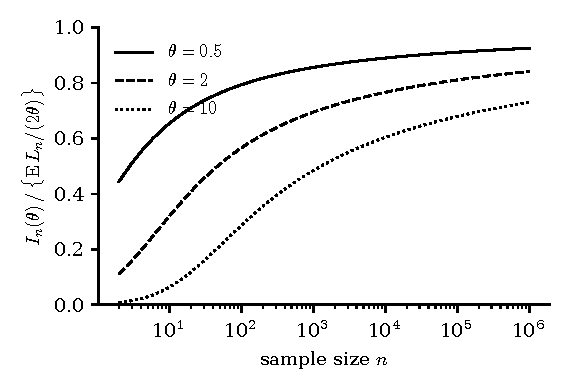
\includegraphics[width=3.8in]{figures/esf_fig_inforatio.pdf}
\caption{The fraction of the oracle tree information retained by the allelic
partition, $I_n(\theta)/\{\E L_n/(2\theta)\}$, against $n$ on a logarithmic scale. The
gap $c(\theta)$ is fixed, so the ratio tends to one, but only at rate $1/\log n$.}
\label{esf:fig:inforatio}
\end{figure}

The estimation problem
is hard because the tree is short. Each new sample member attaches to a genealogy
whose total length is already about $2 \log n$ and lengthens it by only $2/n$, so
doubling the sample adds a fixed quantity of information rather than doubling it.

\subsection{Where the two parameter family leaves the coalescent}

In the Kingman construction the event probabilities depend on the number of active
lineages and on nothing else. Assumption \ref{esf:as:pred2} allows them to depend on
$K_n$, the number of alleles already resolved, which no rate specification in the
lineage count alone can produce. The Kingman genealogy with infinitely many alleles is
therefore exactly the case $\alpha = 0$, and the butterfly estimate
$\hat\alpha = -0.15$ is a statement that the sample is not the allelic partition of
such a model. It does not follow that the genealogy is wrong. The negative branch is
itself a coalescent model, with the infinitude of alleles dropped.

\begin{proposition}[The negative branch is the finite allele model]
\label{esf:prop:kallele}
Let $\alpha = -a < 0$ and $\theta = ma$ with $m$ a positive integer. Then
\eqref{esf:eq:pyeppf} equals the partition law of a sample of size $n$ from $m$ types with
symmetric Dirichlet frequencies $\Dir(a,\dots,a)$, namely
\begin{equation}
m (m-1) \cdots (m-k+1) \; \frac{\prod_{j=1}^{k} (a)_{n_j}}{(ma)_n} ,
\label{esf:eq:dirmult}
\end{equation}
which is the stationary sampling law of the $m$ allele model with parent independent
mutation under a Kingman genealogy.
\end{proposition}

\begin{proof}
Substituting $\alpha = -a$ and $\theta = ma$ in \eqref{esf:eq:pyeppf},
$\prod_{i=1}^{k-1}(\theta + i \alpha) = a^{k-1} \prod_{i=1}^{k-1}(m-i)$, while
$(\theta+1)_{n-1} = (ma)_n / (ma)$ and
$(1-\alpha)_{n_j-1} = (1+a)_{n_j-1} = (a)_{n_j}/a$. Multiplying,
\[
\frac{a^{k-1} \prod_{i=1}^{k-1}(m-i) \cdot ma \cdot a^{-k} \prod_j (a)_{n_j}}{(ma)_n}
= \frac{m (m-1) \cdots (m-k+1) \prod_j (a)_{n_j}}{(ma)_n},
\]
which is \eqref{esf:eq:dirmult}. The right hand side is the Dirichlet multinomial
partition probability obtained by integrating a multinomial sample against a symmetric
$\Dir(a,\dots,a)$ frequency vector and choosing which of the $m$ types the $k$
occupied ones are.
\end{proof}

So the butterflies are not evidence against Kingman's genealogy. They are evidence
against the infinitely many alleles assumption laid on top of it: the fit keeps the
coalescent and replaces the inexhaustible allele space by a finite one of about $1443$
types with per type parameter $0.15$. That is a considerably milder conclusion than
abandoning the genealogical model, and it is the one the data actually support.

For completeness, the remaining branch $0 < \alpha < 1$ does leave the Kingman
genealogy, since no finite type space will produce a power law abundance spectrum. The
natural home for that case is the family of coalescents with multiple mergers
\citep{esf:pitman1999}, in which several lineages may coalesce at once; we do not pursue
the correspondence here, and note only that the butterflies give it no support.

\section{Bayesian inference and prediction}
\label{esf:sec:bayes}

Everything so far has been likelihood based, which understates the case: the whole
construction is a statement about a forecaster's predictive rule, and the natural
summary of what the butterflies say about $\theta$ is a posterior rather than a
standard error. This section supplies one, and then answers Corbet's question with a
predictive distribution rather than a point.

\subsection{Data augmentation for the mutation parameter}

By Corollary \ref{esf:cor:suff} the likelihood is
$L(\theta) \propto \theta^{K_n} \Gamma(\theta)/\Gamma(\theta+n)$, a function of the
data through $K_n$ alone, so the posterior inherits that reduction. The ratio of gamma
functions is awkward, but it has an exact integral representation that makes the
posterior a two block Gibbs sampler.

\begin{proposition}[Beta augmentation]
\label{esf:prop:ew}
For $\theta > 0$ and $n \ge 1$,
\begin{equation}
\frac{\Gamma(\theta)}{\Gamma(\theta+n)}
= \frac{\theta+n}{\theta \, (n-1)!} \int_0^1 \eta^{\theta} (1-\eta)^{n-1} \, d\eta .
\label{esf:eq:betaaug}
\end{equation}
Consequently, under a $\mathrm{Gamma}(a,b)$ prior on $\theta$ with rate $b$, the joint
posterior of $(\theta, \eta)$ given $K_n = k$ satisfies
\begin{align*}
\eta \mid \theta \; &\sim \; \mathrm{Beta}(\theta+1, n), \\
\theta \mid \eta \; &\sim \; \pi_\eta \, \mathrm{Gamma}(a+k, \, c_\eta)
+ (1 - \pi_\eta) \, \mathrm{Gamma}(a+k-1, \, c_\eta),
\end{align*}
where $c_\eta = b - \log \eta$ and
$\pi_\eta / (1-\pi_\eta) = (a+k-1) / (n \, c_\eta)$.
\end{proposition}

\begin{proof}
The Beta integral gives
$\int_0^1 \eta^{\theta}(1-\eta)^{n-1} d\eta = B(\theta+1,n)
= \Gamma(\theta+1)\Gamma(n)/\Gamma(\theta+n+1)$, and
$\Gamma(\theta+1) = \theta \Gamma(\theta)$, $\Gamma(\theta+n+1) = (\theta+n)
\Gamma(\theta+n)$, which rearranges to \eqref{esf:eq:betaaug}. Multiplying the likelihood
by the prior and by the integrand gives joint density proportional to
$\theta^{a+k-2} (\theta+n) e^{-c_\eta \theta} (1-\eta)^{n-1}$, and the bracket
$\theta^{a+k-1} + n \theta^{a+k-2}$ is an unnormalised mixture of the two gamma
densities with the stated odds.
\end{proof}

This is the device of \citet{esf:escobar1995}, where it appears as one node of a
larger sampler for Dirichlet process mixtures \citep{esf:antoniak1974}. Here $\theta$ is the only unknown, so
the posterior is one dimensional and can be obtained by quadrature; we compute it both
ways, which checks the sampler against an exact answer.

For the butterflies $n$ is not observed. Given $n$ the censored likelihood of Section \ref{esf:sec:empirical} is $\theta^{620}\Gamma(\theta)/\Gamma(\theta+n)$ times a factor free of $\theta$, so the proposition applies with $k = 620$ at any fixed $n$; we run the sampler at $n = \hat n = 11068$ and check it against quadrature at the same $n$, and we also report the posterior with $n$ integrated out under a flat prior, by quadrature over $(\theta, n)$.

To see why the sampler mixes well, follow one sweep from $\theta = 142$ with
$n = 11068$, $k = 620$ and the prior $\mathrm{Gamma}(1, 0.01)$ used below. The
augmentation variable has mean $\E(\eta \mid \theta) = 143/11211 = 0.01276$; at that
value $c_\eta = 0.01 - \log 0.01276 = 4.372$, the mixing weight is
$\pi_\eta = 0.013$, and the conditional law of $\theta$ is essentially
$\mathrm{Gamma}(620, 4.372)$, with mean $141.8$ and standard deviation
$\sqrt{620}/4.372 = 5.7$. That conditional spread is most of the posterior standard
deviation of about $6.5$, so successive draws of $\theta$ are only weakly correlated (the lag one autocorrelation is $0.22$)
and a single sweep can move across the bulk of the posterior. Table \ref{esf:tab:post} and the
left panel of Figure \ref{esf:fig:posterior} show that the sampler and quadrature agree to two decimal places in
the mean and to within Monte Carlo error at the quantiles. With $k = 620$ the prior is
irrelevant: a $\mathrm{Gamma}(1, 0.01)$ prior, with mean $100$, moves the posterior
mean to $141.67$ against a maximum likelihood value of $141.75$. Integrating over $n$ lowers the mean slightly and widens the interval a little.

\begin{table}[htbp]
\centering
\caption{Posterior for $\theta$ on Corbet's butterflies under a
$\mathrm{Gamma}(1, 0.01)$ prior, computed two ways at the profiled $n$ and by quadrature with $n$ integrated out under a flat prior, with the maximum likelihood fit
for comparison.}
\label{esf:tab:post}
\begin{adjustbox}{max width=\textwidth}
\begin{tabular}{lrrr}
\toprule
& mean & median & 90 percent interval \\
\midrule
Quadrature, $n = 11068$                     & 141.67 & 141.55 & $(131.23,\ 152.48)$ \\
Beta augmentation, $n = 11068$, $2 \times 10^{5}$ sweeps & 141.67 & 141.54 & $(131.25,\ 152.50)$ \\
Quadrature, $n$ integrated out  & 141.16 & 140.84 & $(129.75,\ 152.66)$ \\
Maximum likelihood, $n$ profiled & 141.75 & & $141.75 \pm 1.645 \times 7.0$ \\
\bottomrule
\end{tabular}
\end{adjustbox}
\end{table}

\begin{figure}[htbp]
\centering
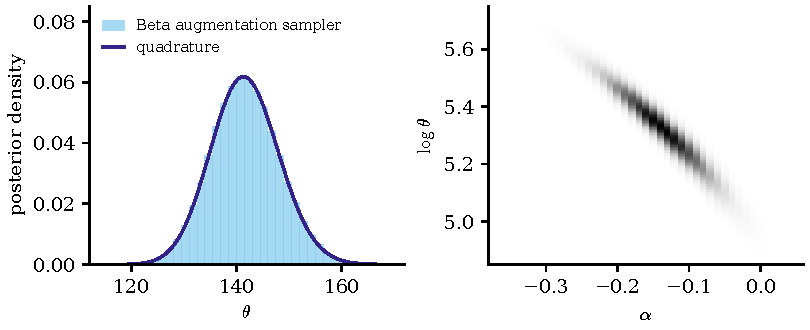
\includegraphics[width=\textwidth]{figures/esf_fig_posterior.pdf}
\caption{Left: posterior for $\theta$ in the Ewens model at $n=\hat n=11068$, quadrature against the Beta augmentation sampler. Right: joint posterior for $(\alpha, \log \theta)$ in the two parameter model, with $n$ integrated out.}
\label{esf:fig:posterior}
\end{figure}

\subsection{The two parameter posterior}

For the two parameter model the likelihood \eqref{esf:eq:pysf} is no longer a function of
$K_n$ alone, and no augmentation of the kind above is available, but the parameter
space is two dimensional and quadrature on a grid is exact enough. Under a uniform
prior on $\alpha$ and on $\log \theta$, restricted to the admissible region, the
posterior is summarised in the right panel of Figure \ref{esf:fig:posterior} and by
\[
\begin{gathered}
\alpha : \ -0.137 \ (-0.23, \, -0.05), \qquad
\theta : \ 206 \ (163, \, 251), \\
m = \theta / |\alpha| : \ 1773 \ (1098, \, 3160),
\end{gathered}
\]
posterior means with ninety percent intervals, $n$ being integrated out under a flat prior. The posterior probability that
$\alpha < 0$ is $0.995$. The evidence for a finite species pool is
therefore not an artefact of maximising, but the pool size is poorly determined: the interval runs from about $1100$ to $3200$ species against the $620$ already seen, and the posterior of $m$ has a long right tail, since $m = \theta/|\alpha|$ grows without bound as $\alpha$ approaches the Ewens value.

\subsection{How many new species?}

Corbet's question was what a second expedition of the same size would add. Under
either model the answer has an exact conditional law. Given $(\alpha, \theta)$ and the
current state, the indicator that individual $i+1$ starts a new species is Bernoulli
with probability $(\theta + \alpha K_i)/(\theta + i)$, so for the Ewens model
$\alpha = 0$ the number of new species in a further $t$ individuals is a sum of
independent Bernoulli variables,
\begin{equation}
K_{n+t} - K_n \; \sim \; \sum_{i=n}^{n+t-1} \mathrm{Bernoulli}
\left( \frac{\theta}{\theta+i} \right),
\label{esf:eq:newspecies}
\end{equation}
free of $K_n$, while for $\alpha \ne 0$ the chain must be run forward because each new
species changes the next probability. Mixing \eqref{esf:eq:newspecies} over the posterior
for $\theta$, and simulating the urn forward under the posterior for
$(\alpha, \theta)$, gives the posterior predictive distributions in Figure
\ref{esf:fig:predictive}:
\[
\text{Ewens: } 97.2 \ (80, \, 116), \qquad
\text{two parameter: } 79.2 \ (60, \, 98),
\]
for a further sample of the same size $n$ as the first, drawn with $n$ from its posterior, against the model free alternating sum of \citet{esf:good1956}, which is $75$ on the
tabulated classes and is the figure Fisher reported.

\begin{figure}[htbp]
\centering
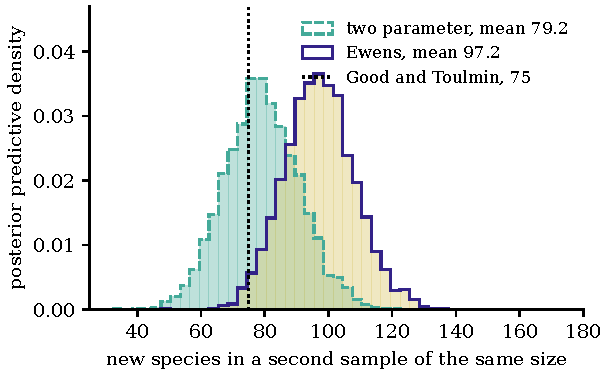
\includegraphics[width=0.75\textwidth]{figures/esf_fig_predictive.pdf}
\caption{Posterior predictive distribution of the number of new species in a further
sample of the same size as the first, under both models, with the Good and Toulmin value
marked.}
\label{esf:fig:predictive}
\end{figure}

The Ewens model assigns
posterior probability $0.98$ to a count exceeding Fisher's own answer, and its ninety
percent interval excludes $75$; the two parameter model puts $75$ near the middle of its predictive distribution, with probability $0.66$ of a count of at least $75$. An inexhaustible
pool is not merely optimistic here, it is hard to reconcile with the nonparametric
extrapolation from the same table, although, as the next example shows, that
extrapolation is itself noisy. The discrepancy is a consequence of the
logarithmic growth $\E K_n \sim \theta \log n$ that Assumption \ref{esf:as:pred} imposes.

\begin{example}[How noisy is the Good and Toulmin figure?]
\label{esf:ex:goodtoulmin}
The alternating sum on Corbet's table is
\[
\begin{aligned}
&118 - 74 + 44 - 24 + 29 - 22 + 20 - 19 + 20 - 15 + 12 - 14 \\
&\quad + 6 - 12 + 6 - 9 + 9 - 6 + 10 - 10 + 11 - 5 + 3 - 3 = 75 .
\end{aligned}
\]
Under the Ewens model at $\hat\theta = 141.75$ and $\hat n = 11068$ its expectation, computed from
\eqref{esf:eq:EAj} over all $j \le n$, is $97.36$, equal to two decimals to the expected
number of new species in a second sample of size $\hat n$; restricted to $j \le 24$ it is $95.2$. So the
alternating sum is, for this model, a nearly unbiased predictor, and the comparison
in the text is fair. It is, however, a noisy one. In $2000$ samples of $n = 11068$
simulated from the urn at $\theta = 142$, the alternating sum over $j \le 24$ had mean
$95.7$ and standard deviation $21.6$, and fell at or below $75$ in $17.7$ percent of
samples. Taken alone, then, the Good and Toulmin figure is no real evidence against
the Ewens model; the main evidence is the likelihood comparison of Table
\ref{esf:tab:fits}, and the predictive comparison should be read as showing that the
two models give materially different answers to Corbet's question, not as an
independent test.
\end{example}

\section{Discussion}
\label{esf:sec:discussion}

\subsection{What each hypothesis contributes}

It is worth separating the three ingredients, because they do very different amounts
of work. Exchangeability alone yields the representation \eqref{esf:eq:definetti} with an
arbitrary mixing measure $\mu$ on $\Fcal$, and that is all it yields; it is far too
weak to produce a sampling formula, and Corollary \ref{esf:cor:df} shows that even its
finite sample content is a statement about $k$ being small relative to $n$ rather than
about the shape of anything. The second ingredient, Assumption \ref{esf:as:pred}, is where
the model enters: the one step forecast is an affine function of the empirical
distribution function with coefficients free of the data. Proposition
\ref{esf:prop:weights} shows that this collapses the whole family of weight sequences to
the single harmonic family indexed by $\theta$, using nothing but the equality of
pairwise tie probabilities. The third ingredient is diffuseness of $H$, which is what
makes ties informative: without it, two observations could agree by landing on a
common atom of the base measure rather than by sharing a type, and the partition would
no longer be the object the sampling formula describes.

In Kingman's language, Assumption \ref{esf:as:pred} selects the Ewens member of the family
of exchangeable partitions, the Gibbs partitions of type zero \citep{esf:gnedin2006}; in genealogical language, by
Proposition \ref{esf:prop:coal}, it selects the Kingman coalescent with killing.
Assumption
\ref{esf:as:pred2} enlarges the selection to the two parameter family by letting the
coefficients see the number of jumps of $F_n$ and by loading the empirical
distribution function of the distinct values alongside $F_n$ itself. Both assumptions
are statements about which functionals of the empirical distribution function the
forecaster is permitted to use, which is the sense in which this chapter treats the
sampling formula as a theorem about $F_n$ rather than about genealogy.

\subsection{The paintbox, Poisson Dirichlet and homozygosity}

By Proposition \ref{esf:prop:dp} and the stick breaking construction of \citet{esf:sethuraman1994}, $\Ptil$ can
be written as $\sum_{\ell \ge 1} p_\ell \delta_{\xi_\ell}$ with $\xi_\ell$ independent
draws from $H$ and $(p_\ell)$ obtained from independent Beta$(1,\theta)$ sticks. The
ranked rearrangement of $(p_\ell)$ has the Poisson Dirichlet law with parameter
$\theta$ \citep{esf:pitman2006}. Conditionally on $\Ptil$ the sequence is independent and identically
distributed, so the partition by ties is exactly Kingman's paintbox applied to that
ranked sequence, and Theorem \ref{esf:thm:esf} recovers the classical statement that the
paintbox of a Poisson Dirichlet frequency vector produces the Ewens sampling formula.

The route taken here reverses the usual order of exposition. The standard development
starts from the frequencies, defines the paintbox, and derives the sampling formula by
combinatorics; the present one starts from the forecaster's rule, derives the sampling
formula by a telescoping product, and arrives at the frequencies only afterwards, as
the atoms of the Helly and Bray limit. The two meet at the homozygosity: the random
quantity $\sum_\ell p_\ell^2$ equals $\PP(X_1 = X_2 \mid \Ptil)$ and has expectation
$1/(1+\theta)$, which is the pairwise tie probability $q$ of Proposition
\ref{esf:prop:weights} and the single number that drove the entire identification
argument. Everything this chapter proves about $\theta$ is, in the end, a restatement of
how often two randomly chosen individuals share a type.

\subsection{Two ways to read the parameter off the empirical distribution function}

Proposition \ref{esf:prop:exactvar} identifies $\theta$ from the heights of $F_n$, exactly
and at every $n$, but it identifies it from a variance, so it requires either
independent replication or knowledge of $H$. Corollary \ref{esf:cor:suff} says that the
jumps alone are sufficient, so a single sample suffices, but it gives up the
connection to the de Finetti limit. The two are complementary rather than competing.
The variance identity is what makes the de Finetti argument close, since it exhibits
$\theta$ as a functional of the object that Helly and Bray produced; $K_n$ is what one
computes from data. Proposition \ref{esf:prop:pyident} shows that in the two parameter
model both are needed at once and neither suffices alone: the heights deliver only
$\rho = (1-\alpha)/(1+\theta)$, and the growth rate of the jump count must supply the
second coordinate.

The estimation problem is genuinely hard in a way the algebra conceals. The
information about $\theta$ grows like $\log n$, so that the standard error in Table
\ref{esf:tab:kn} improves by less than a quarter between $n = 10^{3}$ and $n = 10^{4}$,
and the widely used estimator $K_n/\log n$ carries a bias $-\theta \psi(\theta)/\log n$
of smaller order than its standard deviation yet larger than it at realistic $n$ when $\theta$ is large. At $\theta = 10$ and $n = 10^{4}$ that
bias pulls the estimate down by a quarter of the parameter. Solving the likelihood equation costs nothing and
removes it.

\subsection{Sharpness of the sampling bound}

The bound $2 p_{n,k}$ of Lemma \ref{esf:lem:wor} is of the right order. For $k$ growing
like $\sqrt{n}$ the birthday problem shows that sampling with and without replacement
are not asymptotically equivalent, so no bound of this type can hold beyond that
range; and since de Finetti's theorem is a statement about fixed $k$ and large $n$,
the bound is more than sufficient for Theorem \ref{esf:thm:definetti}. Corollary
\ref{esf:cor:df} records the corresponding statement for finite exchangeable sequences,
recovering the estimate of \citet{esf:diaconis1980} as a by product rather than as
a separate theorem. It is worth noticing that this is the only quantitative inequality
in the entire derivation of the sampling formula: everything else is exact algebra.

\subsection{What the butterflies did and did not settle}

The data were brought in to illustrate the theory and ended by discriminating between
two extensions of it. The one parameter fit misfits in a specific direction, over
predicting the rarest class by about a fifth and under predicting the moderately abundant
classes, though once the censoring of the table is modelled the misfit is modest; that pattern is what an ascertainment story predicts, and it is why Section
\ref{esf:sec:weighted} was written. But the power weighted paintbox cannot produce it: as
Table \ref{esf:tab:weighted} shows, raising $\beta$ buys a lower singleton count only by
lowering the richness in nearly the same proportion, and the data want more species and a flatter
profile simultaneously. The two parameter family delivers both, and it does so on the
negative branch, which by Remark \ref{esf:rem:finite} is not an ascertainment model at all
but a finite pool, estimated at about $1400$ by maximum likelihood and $1800$ by the posterior mean, with a symmetric Dirichlet abundance profile.
The likelihood ratio statistic of $8.57$ is clear evidence but not overwhelming, and Section \ref{esf:sec:bayes} shows the posterior agrees: probability $0.995$
on $\alpha < 0$, a poorly determined pool size, and a predictive interval for the second expedition that covers
Fisher's answer where the Ewens interval misses it.

Two things this does not settle. The comparison is not a like for like test: the
weighted paintbox and the two parameter family are not nested and were compared
informally, by simulation against likelihood, rather than by a common criterion. And
the tabulation is the published one, censored at $j = 24$, so the total sample size is estimated rather than observed; an analysis that treats the $24$ classes as the whole sample gives $\hat\theta = 164$ and a much stronger, but spurious, case against the Ewens model. The
$\hat\theta$ of $142$ reported here should in any case not be compared with the value
near $40$ often quoted as Fisher's $\alpha$, which belongs to the Rothamsted light
trap moths rather than to these butterflies.

\subsection{Open questions}

Four seem worth recording.

First, Proposition \ref{esf:prop:zabell} is stated with a gap. Zabell's theorem
characterises the Dirichlet process among species sampling sequences with an affine
predictive; what is missing is the complementary statement that a nonconstant weight
function actually moves $\Ptil^{\, w}$ off the Dirichlet class. The simulations make
this plain for power weights, but a proof covering all admissible $w$, presumably
through the induced law on ranked frequencies, would let Proposition
\ref{esf:prop:zabell} be stated as the clean dichotomy it appears to be.

Second, the characterisation direction of Assumption \ref{esf:as:pred2} is quoted rather
than proved. The forcing argument of Proposition \ref{esf:prop:weights} is short because
exchangeability of pairwise ties determines everything once the coefficients are
deterministic; when the coefficients are allowed to depend on $K_n$ the same device no
longer closes, since the relevant expectation involves the joint law of the block size
and the jump count. A self contained proof in the style of Proposition
\ref{esf:prop:weights} would complete the parallel between the two assumptions.

Third, the weighted paintbox of \eqref{esf:eq:weighted} and the tilt of Section
\ref{esf:sec:twoparam} are distinct operations on the same object, and nothing forbids
applying both. A weighted two parameter paintbox has three parameters and would let
ascertainment and pool size be estimated jointly rather than compared informally; the
obstacle is \eqref{esf:eq:weppf}, which has no closed form, so the comparison would have
to be made by simulation based inference. A prior question is whether the two operations ever coincide: Proposition \ref{esf:prop:notweighted} shows that no weighted Kingman paintbox has the law of the negative branch, but for $0 < \alpha < 1$ we do not know whether some weight $w$ applied to a Poisson Dirichlet paintbox reproduces the two parameter law exactly.

Fourth, the identification result of Proposition \ref{esf:prop:pyident} is a statement
about two functionals of the limiting empirical distribution function, the variance of
its heights and the growth rate of its jump count. It is natural to ask how far this
goes: for which families of exchangeable partitions is the de Finetti limit identified
by a finite list of such functionals, and is there a general principle assigning one
functional per parameter? The Gibbs partitions of type $\alpha$ \citep{esf:gnedin2006} would be the place
to start.

\section{Exercises}
\label{esf:sec:exercises}

\begin{enumerate}[label=\arabic*., leftmargin=*]

\item Six balls, three of colour $0$ and three of colour $1$, are in an urn. Compute
the exact total variation distance between the laws of the ordered colours of two
balls drawn with and without replacement, and compare it with $p_{6,2}$ and with
$k(k-1)/(2n)$.
\emph{Hint.} The four ordered pairs have probabilities $1/4$ each with replacement and
$1/5, 3/10, 3/10, 1/5$ without; the answer is $1/10$, against $p_{6,2} = 1/6$.

\item Show that for distinct $x_1,\dots,x_n$ the bound of Lemma \ref{esf:lem:wor} is
attained: the total variation distance between the value laws equals $p_{n,k}$. Use
the birthday approximation $p_{n,k} \approx 1 - e^{-k(k-1)/(2n)}$ to find the $k$ at
which it first exceeds one half when $n = 365$.
\emph{Hint.} The value map is one to one on tuples; $k = 23$.

\item Write out the law of the allelic partition for $n = 3$ from
\eqref{esf:eq:esf2}, and verify by expanding that $\E K_3 = 1 + \theta/(\theta+1) +
\theta/(\theta+2)$.
\emph{Hint.} Example \ref{esf:ex:coal3} lists the three probabilities.

\item Prove that at $\theta = 1$ the sampling formula is the law of the cycle type of a
uniform random permutation of $\{1,\dots,n\}$, and deduce that $\E A_j = 1/j$ for
$1 \le j \le n$.
\emph{Hint.} Use \eqref{esf:eq:esfcycle} and, for the mean, \eqref{esf:eq:EAj} with
$\theta = 1$.

\item Show that $\PP(K_n = 1) = (n-1)!/(\theta+1)_{n-1}$ and
$\PP(K_n = n) = \theta^{n-1}/(\theta+1)_{n-1}$, and evaluate both at $n = 5$,
$\theta = 2$.
\emph{Hint.} $s(n,1) = (n-1)!$ and $s(n,n) = 1$ in Corollary \ref{esf:cor:stirling};
the values are $1/15$ and $2/45$, as in Table \ref{esf:tab:small}.

\item Show that the sample homozygosity $\hat F = \sum_j a_j j(j-1)/\{n(n-1)\}$ is
unbiased for $1/(1+\theta)$ under \eqref{esf:eq:esf2}, and compute its variance for
$n = 3$.
\emph{Hint.} $\hat F$ is the proportion of the $\binom{n}{2}$ pairs that are tied, and
each pair is tied with probability $q = 1/(1+\theta)$. For $n = 3$, $\hat F$ takes the
values $1$, $1/3$, $0$ on the three shapes.

\item Prove \eqref{esf:eq:infovar}, $I_n(\theta) = \Var K_n/\theta^{2}$, directly from
the formulas of Proposition \ref{esf:prop:kn}, and explain why the identity must hold
for any family of the form $p_\theta(x) = h(x)\theta^{t(x)}/Z(\theta)$.
\emph{Hint.} Differentiate $\log Z$ twice in $\log\theta$.

\item For Corbet's data, with the censored fit $\hat\theta = 141.75$ and $\hat n = 11068$ of Section \ref{esf:sec:empirical}, show that under the Ewens model the
expected number of new species in a second sample of the same size is
$\sum_{i=n}^{2n-1} \hat\theta/(\hat\theta+i) \approx 97.4$, and compare with the
approximation $\hat\theta \log 2$.
\emph{Hint.} Use \eqref{esf:eq:newspecies}; $141.75 \log 2 = 98.3$, the difference
coming from $\theta$ not being small compared with $n$.

\item In the two parameter model of Assumption \ref{esf:as:pred2} with $n = 3$, show
that the three shapes have probabilities
$(1-\alpha)(2-\alpha)$, $3(1-\alpha)(\theta+\alpha)$ and $(\theta+\alpha)(\theta+2\alpha)$,
each divided by $(\theta+1)(\theta+2)$, and check that they sum to one.
\emph{Hint.} Apply \eqref{esf:eq:pyeppf} and count set partitions of each shape.

\item For the finite pool of Remark \ref{esf:rem:finite} with $m$ types and
concentration $a$, show that
$\E K_n = m\{1 - ((m-1)a)_{n}/(ma)_{n}\}$, where $(x)_n$ is the rising factorial.
Evaluate it at the butterfly fit $m = 1442.6$, $a = 0.1454$, $n = 9747$.
\emph{Hint.} A given type is absent from the sample with probability
$\E(1-P_1)^{n}$, and $1 - P_1 \sim \mathrm{Beta}((m-1)a, a)$; the value is $619.8$,
close to the observed $620$.

\item Show that the total length of the coalescent tree has
$\Var L_n = 4\sum_{k=1}^{n-1} k^{-2}$, so that $L_n/\E L_n \to 1$ in probability, and
compute the mean and variance of the number of mutations $S_n$ on the tree, given
that $S_n$ is Poisson with mean $\theta L_n/2$ conditionally on $L_n$.
\emph{Hint.} $\Var(kT_k) = 4/(k-1)^{2}$; $\E S_n = \theta\sum_{k=1}^{n-1} k^{-1}$ and
$\Var S_n = \E S_n + \theta^{2}\sum_{k=1}^{n-1}k^{-2}$, Watterson's formulas.

\item Simulate Hoppe's urn at $n = 8$, $\theta = 2$ and reproduce Table \ref{esf:tab:esf},
then simulate the coalescent with killing of Section \ref{esf:sec:coalescent} and
check that the two empirical laws of the allelic partition agree.
\emph{Hint.} For the urn, a new allele arrives at step $i+1$ with probability
$\theta/(\theta+i)$; otherwise copy the allele of a uniformly chosen earlier gene.

\end{enumerate}


\begin{thebibliography}{}

\bibitem[Antoniak(1974)]{esf:antoniak1974}
Antoniak, C. E. (1974). Mixtures of Dirichlet processes with applications to Bayesian
nonparametric problems. \textit{The Annals of Statistics} 2, 1152 to 1174.

\bibitem[Arratia, Barbour and Tavar\'e(2003)]{esf:arratia2003}
Arratia, R., Barbour, A. D. and Tavar\'e, S. (2003). \textit{Logarithmic Combinatorial
Structures: A Probabilistic Approach}. Z\"urich: European Mathematical Society.

\bibitem[Blackwell and MacQueen(1973)]{esf:blackwell1973}
Blackwell, D. and MacQueen, J. B. (1973). Ferguson distributions via P\'olya urn
schemes. \textit{The Annals of Statistics} 1, 353 to 355.

\bibitem[Diaconis and Freedman(1980)]{esf:diaconis1980}
Diaconis, P. and Freedman, D. (1980). Finite exchangeable sequences. \textit{The Annals
of Probability} 8, 745 to 764.

\bibitem[Escobar and West(1995)]{esf:escobar1995}
Escobar, M. D. and West, M. (1995). Bayesian density estimation and inference using
mixtures. \textit{Journal of the American Statistical Association} 90, 577 to 588.

\bibitem[Ewens(1972)]{esf:ewens1972}
Ewens, W. J. (1972). The sampling theory of selectively neutral alleles.
\textit{Theoretical Population Biology} 3, 87 to 112.

\bibitem[Ewens(2004)]{esf:ewens2004}
Ewens, W. J. (2004). \textit{Mathematical Population Genetics I: Theoretical
Introduction}, 2nd ed. New York: Springer.

\bibitem[Ferguson(1973)]{esf:ferguson1973}
Ferguson, T. S. (1973). A Bayesian analysis of some nonparametric problems.
\textit{The Annals of Statistics} 1, 209 to 230.

\bibitem[Fisher(1934)]{esf:fisher1934}
Fisher, R. A. (1934). The effect of methods of ascertainment upon the estimation of
frequencies. \textit{Annals of Eugenics} 6, 13 to 25.

\bibitem[Fisher, Corbet and Williams(1943)]{esf:fisher1943}
Fisher, R. A., Corbet, A. S. and Williams, C. B. (1943). The relation between the
number of species and the number of individuals in a random sample of an animal
population. \textit{Journal of Animal Ecology} 12, 42 to 58.

\bibitem[Gnedin and Pitman(2006)]{esf:gnedin2006}
Gnedin, A. and Pitman, J. (2006). Exchangeable Gibbs partitions and Stirling
triangles. \textit{Journal of Mathematical Sciences} 138, 5674 to 5685.

\bibitem[Good and Toulmin(1956)]{esf:good1956}
Good, I. J. and Toulmin, G. H. (1956). The number of new species, and the increase in
population coverage, when a sample is increased. \textit{Biometrika} 43, 45 to 63.

\bibitem[Griffiths(1979)]{esf:griffiths1979}
Griffiths, R. C. (1979). Exact sampling distributions from the infinite neutral
alleles model. \textit{Advances in Applied Probability} 11, 326 to 354.

\bibitem[Heath and Sudderth(1976)]{esf:heath1976}
Heath, D. and Sudderth, W. (1976). De Finetti's theorem on exchangeable variables.
\textit{The American Statistician} 30, 188 to 189.

\bibitem[Hoppe(1984)]{esf:hoppe1984}
Hoppe, F. M. (1984). P\'olya like urns and the Ewens sampling formula.
\textit{Journal of Mathematical Biology} 20, 91 to 94.

\bibitem[Kingman(1978)]{esf:kingman1978}
Kingman, J. F. C. (1978). The representation of partition structures.
\textit{Journal of the London Mathematical Society} 18, 374 to 380.

\bibitem[Kingman(1982a)]{esf:kingman1982a}
Kingman, J. F. C. (1982a). The coalescent. \textit{Stochastic Processes and their
Applications} 13, 235 to 248.

\bibitem[Kingman(1982b)]{esf:kingman1982b}
Kingman, J. F. C. (1982b). On the genealogy of large populations. \textit{Journal of
Applied Probability} 19A, 27 to 43.

\bibitem[Perman, Pitman and Yor(1992)]{esf:perman1992}
Perman, M., Pitman, J. and Yor, M. (1992). Size biased sampling of Poisson point
processes and excursions. \textit{Probability Theory and Related Fields} 92, 21 to 39.

\bibitem[Pitman(1995)]{esf:pitman1995}
Pitman, J. (1995). Exchangeable and partially exchangeable random partitions.
\textit{Probability Theory and Related Fields} 102, 145 to 158.

\bibitem[Pitman(1999)]{esf:pitman1999}
Pitman, J. (1999). Coalescents with multiple collisions. \textit{The Annals of
Probability} 27, 1870 to 1902.

\bibitem[Pitman(2006)]{esf:pitman2006}
Pitman, J. (2006). \textit{Combinatorial Stochastic Processes}. Lecture Notes in
Mathematics 1875. Berlin: Springer.

\bibitem[Pitman and Yor(1997)]{esf:pitmanyor1997}
Pitman, J. and Yor, M. (1997). The two parameter Poisson Dirichlet distribution
derived from a stable subordinator. \textit{The Annals of Probability} 25, 855 to 900.

\bibitem[Rao(1965)]{esf:rao1965}
Rao, C. R. (1965). On discrete distributions arising out of methods of ascertainment.
\textit{Sankhy\=a Series A} 27, 311 to 324.

\bibitem[Sethuraman(1994)]{esf:sethuraman1994}
Sethuraman, J. (1994). A constructive definition of Dirichlet priors.
\textit{Statistica Sinica} 4, 639 to 650.

\bibitem[Zabell(1982)]{esf:zabell1982}
Zabell, S. L. (1982). W. E. Johnson's ``sufficientness'' postulate. \textit{The Annals
of Statistics} 10, 1090 to 1099.

\bibitem[Zabell(1997)]{esf:zabell1997}
Zabell, S. L. (1997). The continuum of inductive methods revisited. In \textit{The
Cosmos of Science} (J. Earman and J. D. Norton, eds.) 351 to 385. Pittsburgh:
University of Pittsburgh Press.

\end{thebibliography}
